\section{Introduction}

From a critical realist perspective, the ERGM results presented in Chapter 6 reflect observed reality. We are dealing with knowledge of what is perceived to be happening \citep{bhaskar2013realist}. Whereas ERGMs are very useful for measuring patterns of perceived social interaction, they do not capture the broader context in which this social interaction occurs. This chapter presents the results from the qualitative analysis of the semi-structured interviews and should shed light on the unmeasured or actual reality, i.e. knowledge of what happens. \medskip

This study employs the agency model proposed by \citet{loyal2001agency} to evaluate the propositions developed in Chapters 2 and 3. The propositions suggest that individuals exchange tacit knowledge to satisfy an innate need for self-determination and because of social expectations or norms. Tempering the decision to share or seek tacit knowledge are external factors such as the presence of boundaries (e.g. organisational, disciplinary, or cultural boundaries), rules of engagement (e.g. contractual arrangements, appropriability regimes), trust (i.e. interpersonal and inter-organisational trust), and power relations (e.g.power-over versus power-to). Skilled brokerage is seen to play a crucial role in helping individuals overcome boundaries, build trust, and manage power relations. The qualitative analysis aims to test the validity of the propositions. \medskip

Unlike the ERGM analysis, which employs deductive logic to test propositions about social interactions, the qualitative analysis uses first- and second-cycle coding to unpack the psychosocial mechanisms that shape tacit knowledge sharing relations in open innovation partnerships. First-cycle coding employs inductive logic to expand a set of provisional codes derived from the propositions into sub-codes that unpack how different social mechanisms operate in practice (see Table \ref{tab:provcode} for the list of the provisional codes). Second-cycle coding uses the logic of retroduction to group the sub-codes into categorical codes. The categorical codes refer to the main components of the \citet{loyal2001agency}'s agency model. \medskip

To get a better sense of the participants interviewed and the weight of their opinions or views, this chapter begins by introducing the interviewees in terms of their role in their respective open innovation partnership, self-reported personal information, and position in their respective knowledge-sharing networks. The chapter then presents the results of the first- and second-cycle coding for each case before concluding with a summary of the leading social mechanisms at play in each partnership.

\begin{table}[]
\centering
\caption[Provisional codes]{Provisional codes derived from theoretical propositions.}
\label{tab:provcode}
%\renewcommand{\arraystretch}{1.2}
\resizebox{0.9\textwidth}{!}{%	
\begin{tabular}{l p{0.4\linewidth}}
\toprule
\multicolumn{1}{c}{Proposition} & \multicolumn{1}{c}{Provisional codes} \\ \midrule
\multirow{2}{*}{\begin{minipage}{0.7\linewidth}
\begin{enumerate}
    \item[1a] Open innovation requires practitioners to connect across real and perceived boundaries to apply their know-how in novel ways.
\end{enumerate}
\end{minipage}} & Real and perceived boundaries \\
 & Doing something novel \\ \\ 
\multirow{2}{*}{\begin{minipage}{0.7\linewidth}
\begin{enumerate}
    \item[1b] Reducing cognitive distance between open innovation partners requires significant social interaction to support learning and the application of knowledge in practice.
\end{enumerate}
\end{minipage}} & Learning \\ 
& Applying knowledge in practice \\ \\ \\
\multirow{2}{*}{\begin{minipage}{0.7\linewidth}
\begin{enumerate}
    \item[2a] Successful open innovation requires a combination of skilled brokerage and network closure.
\end{enumerate}
\end{minipage}} & Brokering exchanges \\
& Collaborating \\ \\ 
\multirow{2}{*}{\begin{minipage}{0.7\linewidth}
\begin{enumerate}
    \item[3a] Formal structures inhibit tacit knowledge exchange in open innovation partnerships.
\end{enumerate}
\end{minipage}} & Rules of engagement \\
& Power structures \\ \\
\multirow{3}{*}{\begin{minipage}{0.7\linewidth}
\begin{enumerate}
    \item[3b] Individual needs dispositions and internalised social norms moderate a person's willingness to seek out or share tacit knowledge.
\end{enumerate}
\end{minipage}} & Satisfying innate needs \\
& Expressing a particular worldview \\
& Identifying with a distinct group \\ \\
\multirow{1}{*}{\begin{minipage}{0.7\linewidth}
\begin{enumerate}
    \item[4a] Reciprocity and closure in tacit knowledge exchange networks indicate high levels of trust in open innovation partnerships.
\end{enumerate}
\end{minipage}} & Trust relations \\ \\  \\
 \multirow{2}{*}{\begin{minipage}{0.7\linewidth}
 \begin{enumerate}
    \item[4b] Who people choose to empower with their know-how depends on how much they trust the receiver to use their know-how in mutually beneficial ways.
\end{enumerate} 
 \end{minipage}}
& Empowering others \\
& Selective revealing \\  \\ \bottomrule
\end{tabular}
}
\end{table}

\section{Participant information}

One aim of the qualitative analysis was to interview a cross-section of participants in terms of their partner affiliation and knowledge network centrality (i.e. central and peripheral actors in the knowledge provider networks). Unfortunately, some targeted participants were either not available or unwilling to be interviewed. Despite not being able to interview all the targeted people, participants who were eventually interviewed revealed much about the social dynamics in each partnership. The interviews covered 33\% of Case 1 participants, 32\% of Case 2 participants, and 17.5\% of Case 3 participants. Most of the participants interviewed reside in Australia. Of the 21 interviews conducted, 13 were face-to-face and the rest done via video-link. Two participants who live abroad were interviewed face-to-face while visiting Australia. \medskip

Table \ref{tab:interviewees} provides a breakdown of the participants interviewed in each case. Interviews ranged from 25 to 106 minutes in duration. Longer interviews tend to bias the qualitative analysis (such interviews are assigned more codes). The longer interviews usually involved participants with higher network centrality. Their privileged network position meant they were well-placed to provide useful information about knowledge exchanges. \medskip

\begin{sidewaystable}[p]
\centering
\caption[Details about each interview]{Details about each interview.}
\label{tab:interviewees}
\resizebox{\textwidth}{!}{%       
\begin{threeparttable}
\begin{tabular}{crrcrc l ccccccccc}
\toprule

& \specialcell[t]{Network\\Id} &
\specialcell[t]{Employer} &
\specialcell[t]{Date of\\interview} &
\specialcell[t]{Duration\\(MM:SS)} &
\specialcell[t]{Interview\\mode} &
\multicolumn{1}{c}{Role} &
\specialcell[t]{Gender} &
\specialcell[t]{Age} &
\specialcell[t]{Education\\level} &
\specialcell[t]{Relevant\\experience\\(years)} &
\specialcell[t]{Job tenure\\(years)} &
\specialcell[t]{Openness} &
\specialcell[t]{Network\\centrality} &
\specialcell[t]{Country} \\ 
\midrule
\multirow{6}{*}{\rotatebox[origin=c]{90}{Case 1} \rotatebox[origin=c]{90}{($n = 18$)}} 
& 1/1 & 1/1 & 18.12.2015 & 79:04 & F2F & General Manager & M & 54 & 6 & 9 & 4 & 0.44 & 31 & AU \\
& 3/1 & 1/1 & 26.04.2016 & 33:34 & F2F & Transport Manager & M & 51 & 2 & 10 & 19 & 0.61 & 18 & AU \\
& 8/1 & 2/1 & 11.03.2016 & 81:01 & F2F & Company Director & M & 62 & 3 & 12 & 12 & 0.78 & 12 & AU \\
& 10/1 & 3/1 & 07.03.2016 & 58:46 & F2F & Director International Sales & M & 44 & 7 & 16 & 9 & 0.72 & 2 & USA \\
& 15/1 & 7/1 & 25.02.2016 & 66:29 & F2F & Research Engineer & M & 51 & 7 & 25 & 1 & 0.72 & 11 & AU \\
& 16/1 & 7/1 & 07.09.2016 & 43:35 & F2F & Research Group Leader & M & 53 & 8 & 16 & 1 & 0.50 & 9 & AU \\ 
\midrule
\multirow{8}{*}{\rotatebox[origin=c]{90}{Case 2} \rotatebox[origin=c]{90}{($n = 25$)}} 
& 1/2 & 1/2 & 01.03.2016 & 59:21 & F2F & Dairy Farmer & M & 28 & 6 & 7 & 7 & 0.44 & 39 & AU \\
& 8/2 & 2/2 & 18.03.2016 & 70:02 & VL & Research Project Leader & F & 41 & 8 & 14 & 10 & 0.50 & 28 & AU \\
& 9/2 & 3/2 & 20.03.2016 & 106:10 & F2F & Farm Systems Manager & M & 46 & 6 & 18 & 8 & 0.78 & 40 & NZ \\
& 10/2 & 4/2 & 18.03.2016 & 48:44 & VL & Technical Specialist & M & 32 & 8 & 10 & 2 & 0.61 & 18 & AU \\
& 11/2 & 5/2 & 04.03.2016 & 66:04 & F2F & Pasture Specialist & M & 58 & 6 & 25 & 8 & 0.78 & 11 & AU \\
& 15/2 & 7/2 & 03.11.2016 & 76:13 & F2F & Company Director & M & 50 & 4 & 25 & 19 & 0.50 & 34 & AU \\
& 18/2 & 3/2 & 16.02.2016 & 69:02 & VL & Executive Oversight & M & 68 & 5 & 35 & 5 & 0.44 & 26 & NZ \\ 
& 23/2 & 3/2 & 11.03.2016 & 24:53 & VL & Technical Specialist & M & 44 & 3 & 25 & 20 & 0.67 & 15 & SE \\ 
\midrule
\multirow{7}{*}{\rotatebox[origin=c]{90}{Case 3} \rotatebox[origin=c]{90}{($n = 40$)}} 
& 9/3 & 9/3 & 14.12.2016 & 61:35 & VL & Research Scientist & M & 50 & 8 & 26 & 26 & 0.61 & 18 & BR \\
& 10/3 & 10/3 & 16.03.2016 & 89:26 & F2F & Research Leader & M & 45 & 8 & 8 & 3 & 0.78 & 70 & AU \\
& 13/3 & 10/3 & 13.05.2016 & 35:42 & F2F & Project Coordinator & F & 41 & 8 & 4 & 4 & 0.72 & 35 & AU \\
& 16/3 & 10/3 & 12.09.2016 & 73:23 & F2F & Technical Specialist & M & 47 & 7 & 16 & 9 & 0.89 & 23 & AU \\ 
& 22/3 & 10/3 & 19.09.2016 & 47:48 & VL & Executive Oversight & M & 61 & 8 & 32 & 32 & 0.53 & 10 & AU \\ 
& 39/3 & 7/3 & 09.09.2016 & 27:14 & VL & Technical Specialist & M & 30 & 7 & 4 & 2 & 0.61 & 10 & MX \\
& 41/3 & 1/3 & 07.10.2016 & 32:36 & VL & Technical Specialist & M & 24 & 6 & 5 & 4 & 0.78 & 3 & NZ \\
\bottomrule
\end{tabular}
\begin{tablenotes}
% \footnotesize
\item[i] $n$ refers to the number of respondents to the online survey.
\item[ii] Education level is based on the Australian Standard Classification for Education, ranging from 2 (secondary education) to 8 (doctoral qualification).
\item[iii] F2F refers to face-to-face interviews, whereas VL refers to \texttt{Skype}\texttrademark\ interviews. 
\item[iv] Network centrality refers to number of incoming and outgoing social ties in the combined (tacit and explicit) knowledge network.
\end{tablenotes}
\end{threeparttable}
}
\end{sidewaystable}


\begin{table}[]
\centering
\caption[Breakdown of sentiment]{Breakdown of sentiment by interviewee. Participants in Case 1 are generally quite positive, unlike the other two cases, where the less positive sentiment is an indicator of some tension in these cases.}
\begin{subtable}{1\textwidth}
\centering
\resizebox{\textwidth}{!}{%   
\begin{tabular}{r *{4}{c}}
\toprule
\multicolumn{1}{c}{}
Network id & Very negative & Moderately negative & Moderately positive & Very positive \\ \midrule
1/1 & \gradientcell{24}{0}{50}{lime}{red}{90} & \gradientcell{26}{0}{50}{lime}{red}{90} & \gradientcell{46}{0}{50}{lime}{red}{90} & \gradientcell{13}{0}{50}{lime}{red}{90} \\
3/1 & \gradientcell{2}{0}{50}{lime}{red}{90} & \gradientcell{4}{0}{50}{lime}{red}{90} & \gradientcell{19}{0}{50}{lime}{red}{90} & \gradientcell{14}{0}{50}{lime}{red}{90} \\
8/1 & \gradientcell{16}{0}{50}{lime}{red}{90} & \gradientcell{23}{0}{50}{lime}{red}{90} & \gradientcell{37}{0}{50}{lime}{red}{90} & \gradientcell{12}{0}{50}{lime}{red}{90} \\
10/1 & \gradientcell{14}{0}{50}{lime}{red}{90} & \gradientcell{13}{0}{50}{lime}{red}{90} & \gradientcell{45}{0}{50}{lime}{red}{90} & \gradientcell{22}{0}{50}{lime}{red}{90} \\
15/1 & \gradientcell{11}{0}{50}{lime}{red}{90} & \gradientcell{18}{0}{50}{lime}{red}{90} & \gradientcell{35}{0}{50}{lime}{red}{90} & \gradientcell{10}{0}{50}{lime}{red}{90} \\
16/1 & \gradientcell{6}{0}{50}{lime}{red}{90} & \gradientcell{8}{0}{50}{lime}{red}{90} & \gradientcell{28}{0}{50}{lime}{red}{90} & \gradientcell{9}{0}{50}{lime}{red}{90} \\ \bottomrule
\end{tabular}
}%
\bigskip
\caption{Case 1}
\label{tab:sentiment_case_1}
\end{subtable}

\bigskip
\begin{subtable}{1\textwidth}
\centering
\resizebox{\textwidth}{!}{%   
\begin{tabular}{r *{4}{c}}
\toprule
\multicolumn{1}{c}{}
Network id & Very negative & Moderately negative & Moderately positive & Very positive \\ \midrule
1/2 & \gradientcell{16}{0}{80}{lime}{red}{90} & \gradientcell{28}{0}{80}{lime}{red}{90} & \gradientcell{27}{0}{80}{lime}{red}{90} & \gradientcell{17}{0}{80}{lime}{red}{90} \\
8/2 & \gradientcell{11}{0}{80}{lime}{red}{90} & \gradientcell{17}{0}{80}{lime}{red}{90} & \gradientcell{33}{0}{80}{lime}{red}{90} & \gradientcell{23}{0}{80}{lime}{red}{90} \\
9/2 & \gradientcell{30}{0}{80}{lime}{red}{90} & \gradientcell{27}{0}{80}{lime}{red}{90} & \gradientcell{72}{0}{80}{lime}{red}{90} & \gradientcell{18}{0}{80}{lime}{red}{90} \\
10/2 & \gradientcell{6}{0}{80}{lime}{red}{90} & \gradientcell{6}{0}{80}{lime}{red}{90} & \gradientcell{42}{0}{80}{lime}{red}{90} & \gradientcell{11}{0}{80}{lime}{red}{90} \\
11/2 & \gradientcell{23}{0}{80}{lime}{red}{90} & \gradientcell{22}{0}{80}{lime}{red}{90} & \gradientcell{44}{0}{80}{lime}{red}{90} & \gradientcell{22}{0}{80}{lime}{red}{90} \\
15/2 & \gradientcell{25}{0}{80}{lime}{red}{90} & \gradientcell{39}{0}{80}{lime}{red}{90} & \gradientcell{41}{0}{80}{lime}{red}{90} & \gradientcell{22}{0}{80}{lime}{red}{90} \\
18/2 & \gradientcell{8}{0}{80}{lime}{red}{90} & \gradientcell{8}{0}{80}{lime}{red}{90} & \gradientcell{42}{0}{80}{lime}{red}{90} & \gradientcell{15}{0}{80}{lime}{red}{90} \\
23/2 & \gradientcell{2}{0}{80}{lime}{red}{90} & \gradientcell{3}{0}{80}{lime}{red}{90} & \gradientcell{10}{0}{80}{lime}{red}{90} & \gradientcell{5}{0}{80}{lime}{red}{90} \\ \bottomrule
\end{tabular}
}%
\bigskip
\caption{Case 2}
\label{tab:sentiment_case_2}
\end{subtable}

\bigskip
\begin{subtable}{1\textwidth}
\centering
\resizebox{\textwidth}{!}{%   
\begin{tabular}{r *{4}{c}}
\toprule
\multicolumn{1}{c}{}
Network id & Very negative & Moderately negative & Moderately positive & Very positive \\ \midrule
9/3 & \gradientcell{2}{0}{70}{lime}{red}{90} & \gradientcell{6}{0}{70}{lime}{red}{90} & \gradientcell{12}{0}{70}{lime}{red}{90} & \gradientcell{5}{0}{70}{lime}{red}{90} \\
10/3 & \gradientcell{15}{0}{70}{lime}{red}{90} & \gradientcell{24}{0}{70}{lime}{red}{90} & \gradientcell{66}{0}{70}{lime}{red}{90} & \gradientcell{28}{0}{70}{lime}{red}{90} \\
13/3 & \gradientcell{7}{0}{70}{lime}{red}{90} & \gradientcell{11}{0}{70}{lime}{red}{90} & \gradientcell{21}{0}{70}{lime}{red}{90} & \gradientcell{5}{0}{70}{lime}{red}{90} \\
16/3 & \gradientcell{14}{0}{70}{lime}{red}{90} & \gradientcell{19}{0}{70}{lime}{red}{90} & \gradientcell{47}{0}{70}{lime}{red}{90} & \gradientcell{22}{0}{70}{lime}{red}{90} \\
22/3 & \gradientcell{13}{0}{70}{lime}{red}{90} & \gradientcell{12}{0}{70}{lime}{red}{90} & \gradientcell{23}{0}{70}{lime}{red}{90} & \gradientcell{15}{0}{70}{lime}{red}{90} \\
39/3 & \gradientcell{1}{0}{70}{lime}{red}{90} & \gradientcell{4}{0}{70}{lime}{red}{90} & \gradientcell{2}{0}{70}{lime}{red}{90} & \gradientcell{2}{0}{70}{lime}{red}{90} \\
41/3 & \gradientcell{5}{0}{70}{lime}{red}{90} & \gradientcell{4}{0}{70}{lime}{red}{90} & \gradientcell{11}{0}{70}{lime}{red}{90} & \gradientcell{7}{0}{70}{lime}{red}{90} \\ \bottomrule
\end{tabular}
}%
\bigskip
\caption{Case 3}
\label{tab:sentiment_case_3}
\end{subtable}
\end{table}

\begin{figure}
\centering
\begin{subfigure}[b]{0.7\textwidth}
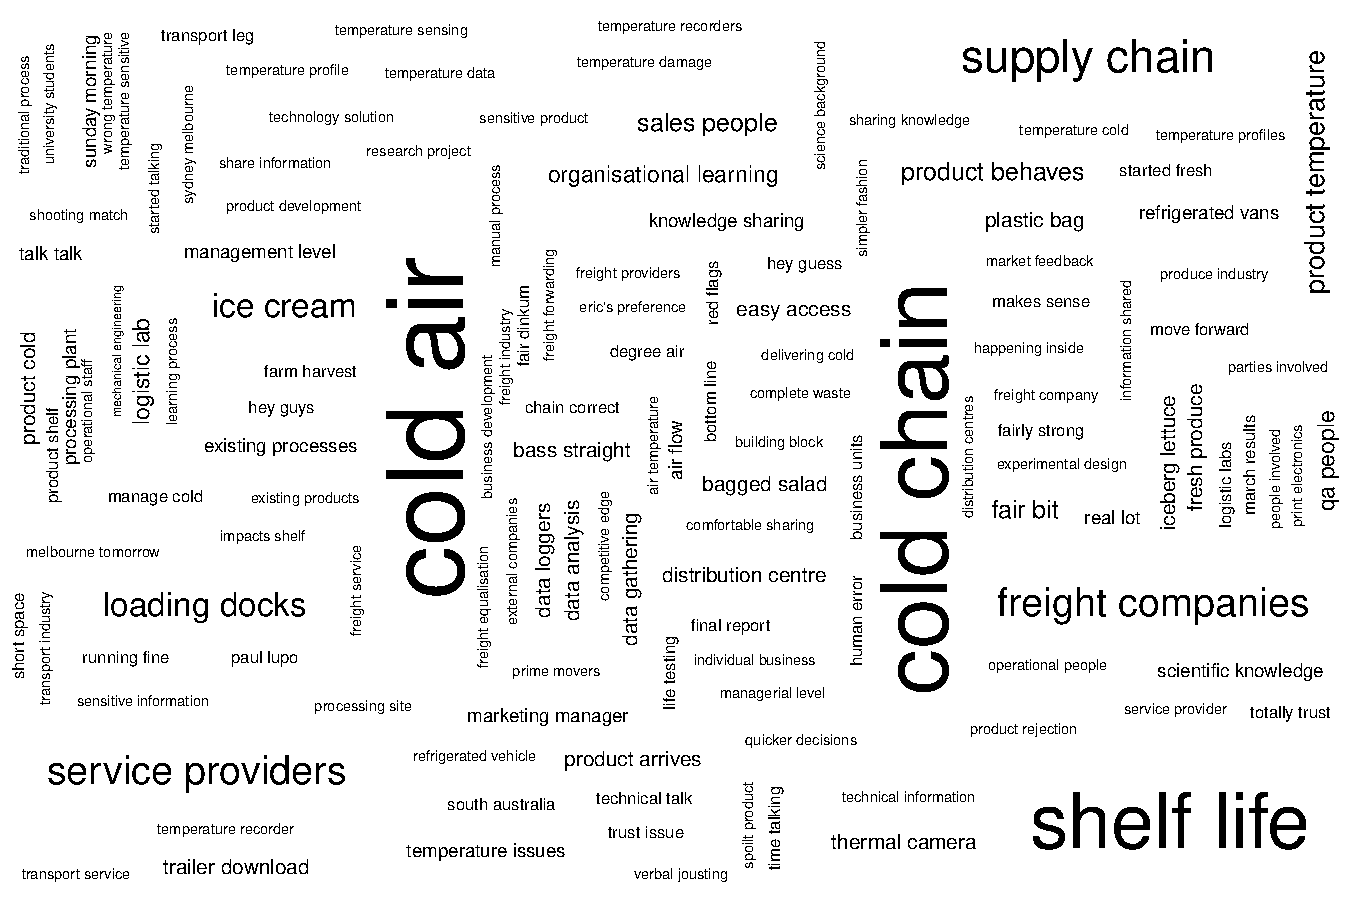
\includegraphics[width=1\linewidth]{Images/bigram_c1.pdf}
\caption{Case 1}
\label{fig:bigram_case_1} 
\end{subfigure}
\bigskip
\begin{subfigure}[b]{0.7\textwidth}
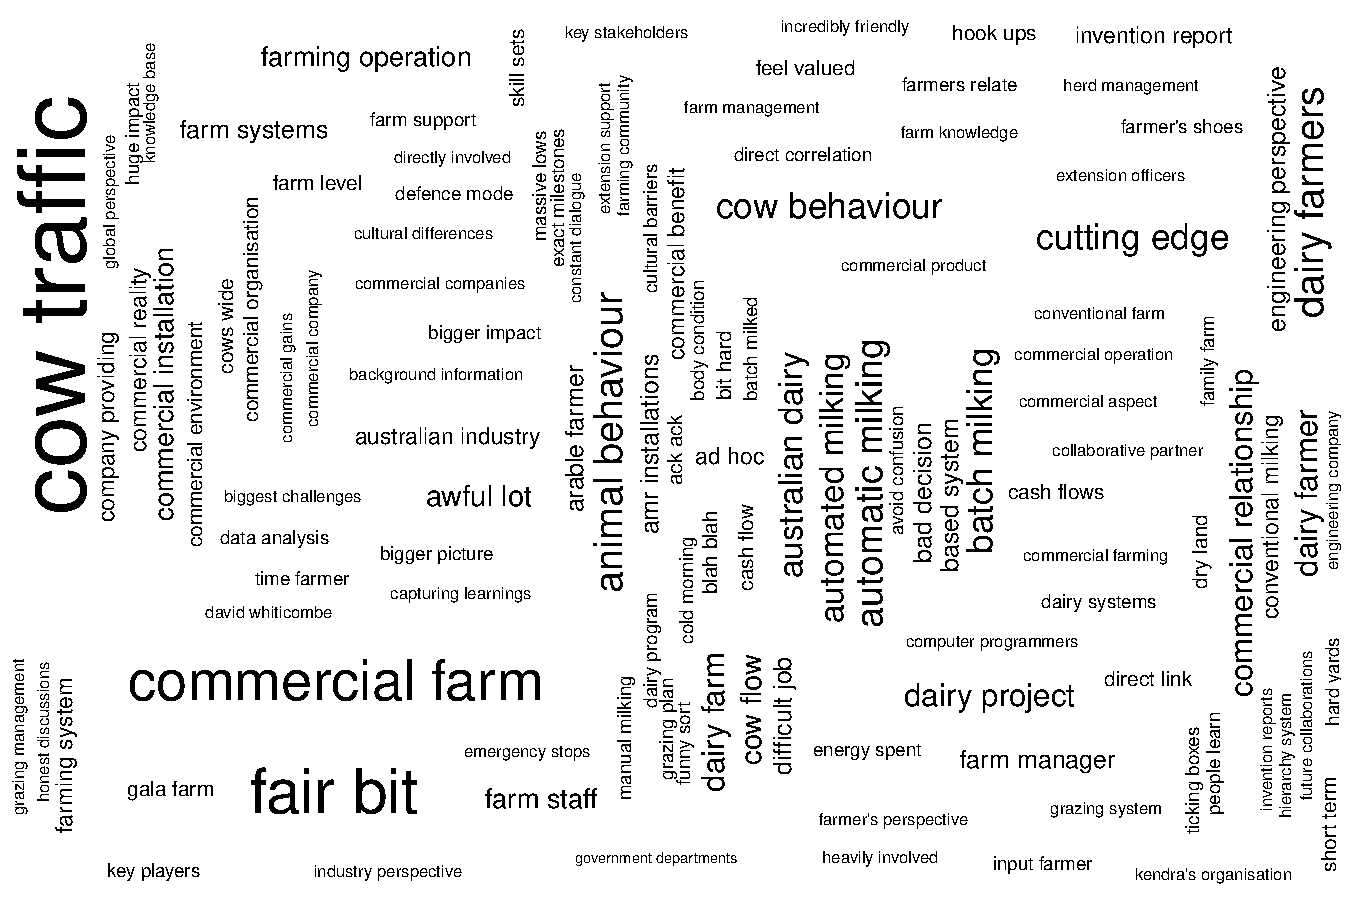
\includegraphics[width=1\linewidth]{Images/bigram_c2.pdf}
\caption{Case 2}
\label{fig:bigram_case_2}
\end{subfigure}
\bigskip
\begin{subfigure}[b]{0.7\textwidth}
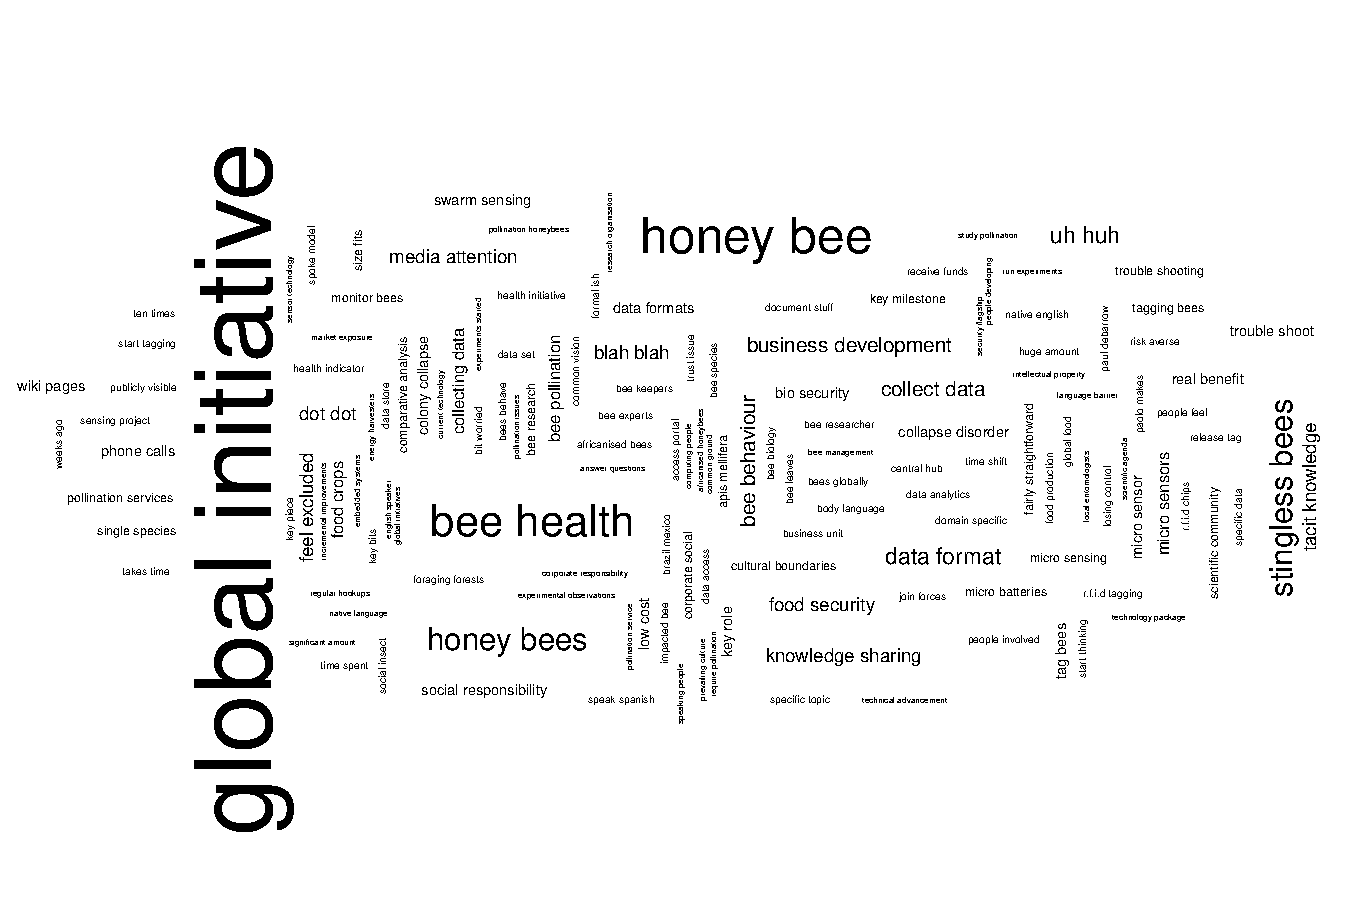
\includegraphics[width=1\linewidth]{Images/bigram_c3.pdf}
\caption{Case 3}
\label{fig:bigram_case_3}
\end{subfigure}
\caption[Bigram word-clouds from interviews]{Bigram word-clouds highlighting what interviewees from each case mainly spoke about.}
\label{fig:bigrams}
\end{figure}


\section{Case 1}

\subsection{Semi-structured interviews}

Six people were interviewed face-to-face in Case 1 (Table \ref{tab:interviewees}). Due to scheduling conflicts, it took nine months to complete all the interviews. The length of the interviews ranged between 34 and 81 minutes (the average interview duration was 60 minutes). Table \ref{tab:sentiment_case_1} shows the overall sentiment expressed by interviewees from Case 1. Most of them were positive about the open innovation partnership. Figure \ref{fig:bigram_case_1} highlights what the interviewees mainly spoke about. Topics that stand out include \enquote{cold air}, \enquote{cold/supply chain}, \enquote{shelf-life}, and \enquote{freight companies}.

\subsection{Recap of network analysis}

The tacit knowledge provider network is quite sparse, suggesting that tacit knowledge is not important in Case 1. The ERGM results indicate people are more likely to share tacit knowledge with others in their immediate social group. Receivers of tacit knowledge tend to be trusted, open to experience, and autonomously motivated. Geography is a limiting factor for tacit knowledge exchanges. Explicit knowledge mostly flows to a few central actors who are likely to be from the same organisation. Providers of explicit knowledge tend to have been in their jobs for some time. \medskip

The modelling of broker roles shows that the representative broker role dominates tacit knowledge exchanges. Explicit knowledge exchanges are more likely to involve liaison brokers (Table \ref{tab:ergm_3}). Whereas the modelling assesses whether broker roles are under or over-represented for all possible two-path configurations, the raw broker counts presented in Figure \ref{fig:gf_c1} allow one to assess dominant brokers in the network. For example, Participant 1/1 stands out as the dominant broker, acting primarily in a liaison and gatekeeper role in the explicit knowledge network and a lesser extent in a representative and internal coordinator role in the tacit knowledge network. Responses to semi-structured interview questions help us understand how Participant 1/1 influenced knowledge flows in both networks.  

\begin{figure}
\centering
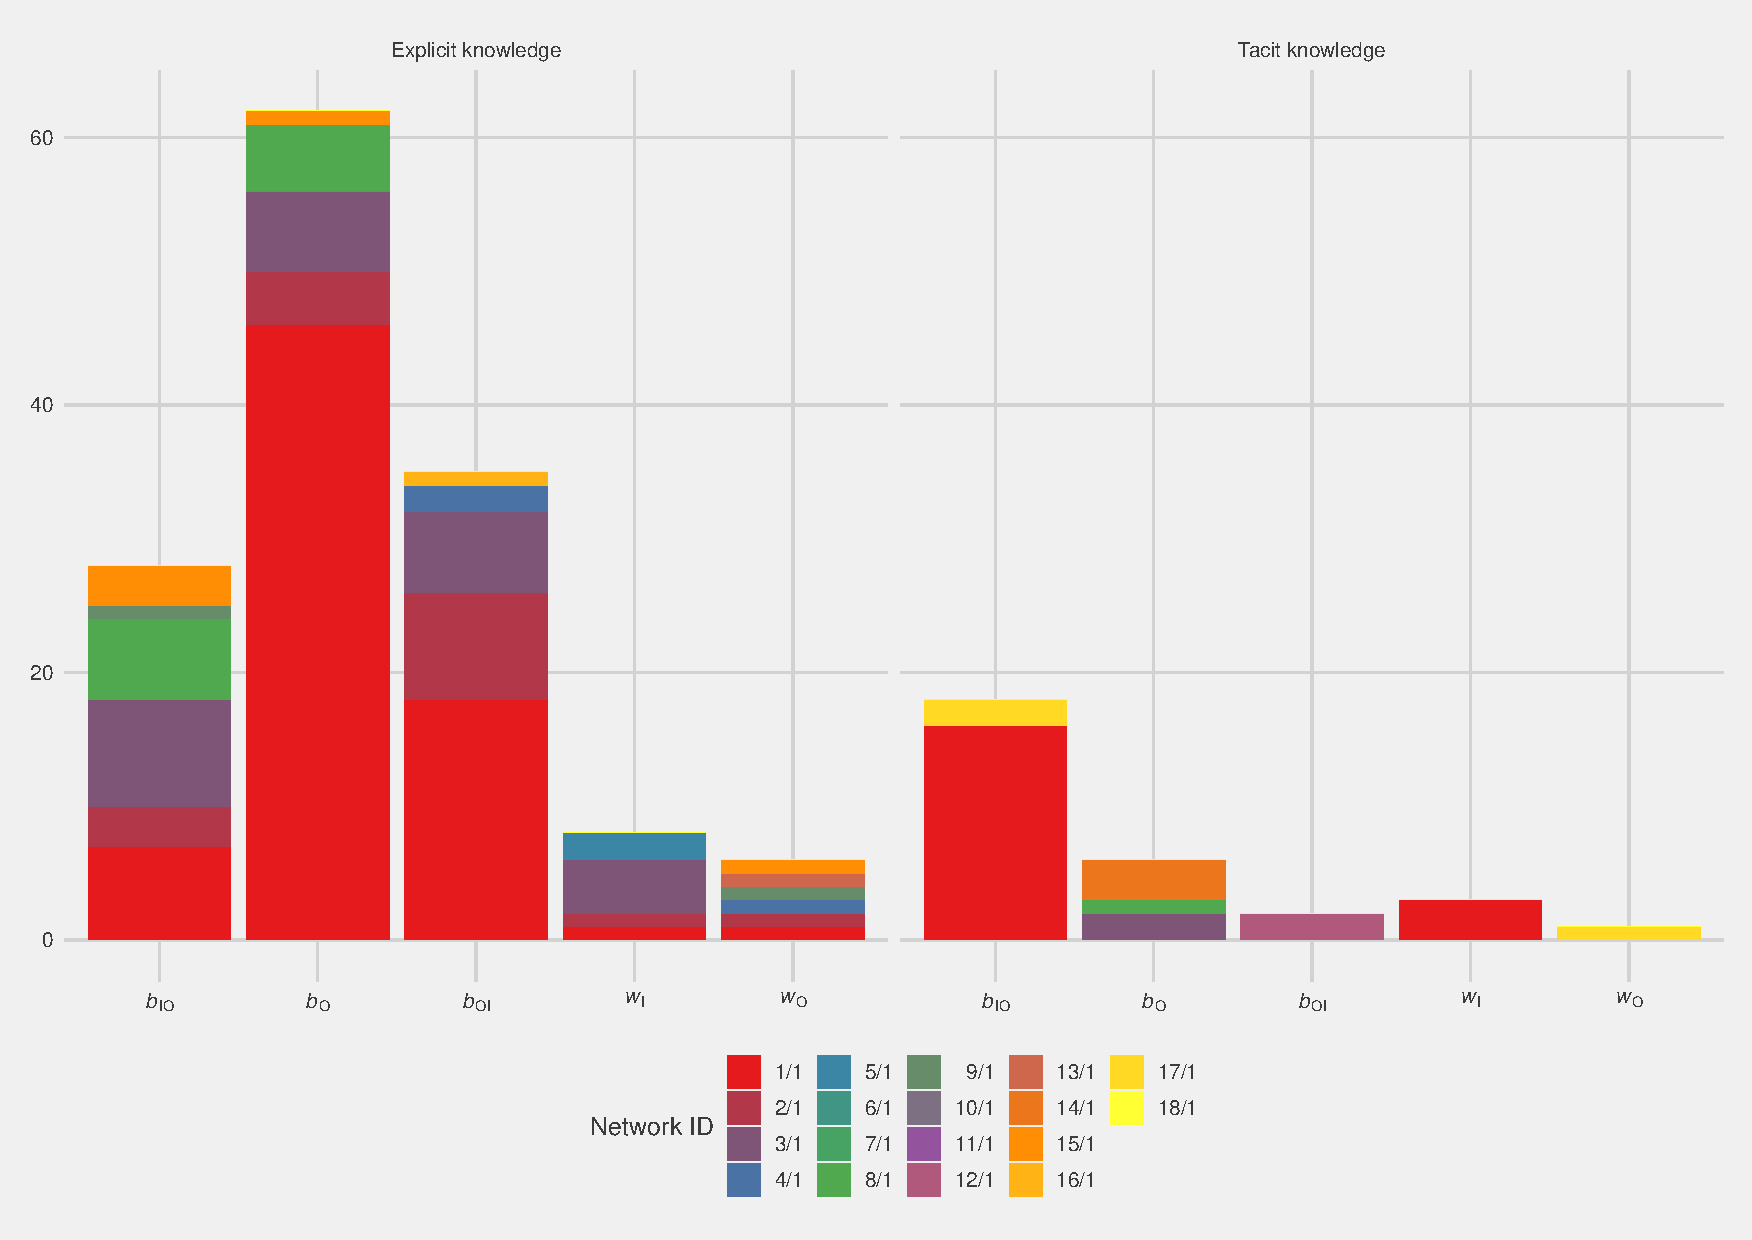
\includegraphics[width = \textwidth]{Images/gf_case1.pdf}
\caption[Breakdown of broker roles by participant in Case 1]{Breakdown of broker roles by participant in Case 1. Note $w_I$ = internal coordinator role, $b_O$ = liaison role, $b_{OI}$ = gatekeeper role, $b_{IO}$ = representative role, and $w_O$ = itinerant broker role. Participant 1/1 stands out as a dominant broker.}
\label{fig:gf_c1}
\end{figure}

\subsection{Coding results}

Table \ref{tab:case_1_codes} lists the most referenced codes in each category for Case 1. Innate needs and subjective norms did not feature strongly in responses to interview questions. Nonetheless, the desire to perform interesting and meaningful work was an important motivator. However, the sharing of know-how appears to be tempered by participants with a narrow outlook, who resist change, or consider themselves intellectually superior to others. Key mechanisms and structures moderating tacit knowledge exchanges include the need to have good relations to facilitate open and honest discussions, swift trust, difficulty accessing knowledgeable people and poor communication. Actions revolved around broadening understanding to improve practices, tapping external expertise, and brokering (or restricting) knowledge exchanges. 

\begin{sidewaystable}
\centering
\caption{Top codes in each category: Case 1.}
\label{tab:case_1_codes}
\begin{tabular}{lllc}
\toprule
Category code & Provisional code & Detailed code & References \\ 
\midrule
Innate needs & Motivational forces & Desire to do meaningful work &   5 \\
Subjective norms & Expressing a particular worldview & Maintaining a narrow perspective &   6 \\ 
Subjective norms & Expressing a particular worldview & Superior attitude &   4 \\ 
Subjective norms & Expressing a particular worldview & Resisting change &   3 \\ 
Mechanisms \& structures & Trust relations & Having good relations &  10 \\ 
Mechanisms \& structures & Trust relations & Having open and honest discussions &  10 \\ 
Mechanisms \& structures & Trust relations & Swift trust &   9 \\ 
Mechanisms \& structures & Boundaries & Engaging with busy people &   9 \\ 
Mechanisms \& structures & Boundaries & Poor communication &   8 \\ 
Action & Applying knowledge in practice & Improving practices &  30 \\ 
Action & Brokering exchanges & Liaison brokerage &  17 \\ 
Action & Learning & Broaden understanding &  16 \\ 
Action & Learning & Tapping external expertise &  15 \\ 
Action & Brokering exchanges & Gate-keeping &  11 \\ 
\bottomrule
\end{tabular}
\end{sidewaystable}

\subsubsection{Innate needs}

Although the social network analysis suggests receivers of tacit knowledge tend to be autonomously motivated people, the need for competence, autonomy, or social connectedness did not feature strongly in the responses to interview questions. Only the university participants stated they were motivated by a desire to do meaningful and exciting work:

\begin{quote}
\small
\enquote{being seen to be involved in [a particular region] with a major producer out there doing things, hopefully producing something that is meaningful.} \\
\rightline{\rm --- Participant 15/1}
\end{quote}

\begin{quote}
\small
\enquote{I think for any researcher, if you think the work that you do will actually be utilised and you can see evidence of it, well that’s a pretty big kick.} \\
\rightline{\rm --- Participant 16/1}
\end{quote}

\subsubsection{Subjective norms}

The interviews reveal doubts about the absorptive capacity of the refrigerated transport companies. A couple of the interviewees did not believe the freight companies would be able to grasp scientific ideas:

\begin{quote}
\small
\enquote{I don't think they ever look at it scientifically, I think they just look at it very broadly, and that's as far as they go.} \\
\rightline{\rm --- Participant 1/1}
\end{quote}

\begin{quote}
\small
\enquote{if you were talking to [the freight company] yeah, you don't want to start talking about thermal masses and all that sort of stuff.} \\
\rightline{\rm --- Participant 15/1}
\end{quote}

Not wanting to explain things in any great detail denied the freight companies the opportunity to learn more about thermodynamics, which is disappointing given the owner of the main freight company had a strong desire to learn about and implement good cold chain practices:

\begin{quote}
\small
\enquote{ I've always been very, very conscious, and maybe fanatical about having facilities that can keep product cold ... so with that you learn about air flow, and cold air and what's best and what’s not best, and you take advice from people who make the fridges, and who make the vans, and who talk about insulation ... for the last 22 or 23 years of my life I've [been a student of] refrigerated transport.} \\
\rightline{\rm --- Participant 8/1}
\end{quote}

\begin{quote}
\small
\enquote{the guy who we spoke to was the owner [of the freight company] - he was really interested. So I think what happened was that there was an interest level that was really driving it more than anything else.} \\
\rightline{\rm --- Participant 16/1}
\end{quote}

The big supermarket customers are quite prescriptive in how they work with their suppliers. The general manager driving the cold chain initiative was afraid that his supermarket customers would not be receptive to any suggested changes to the way orders are handled:

\begin{quote}
\small
\enquote{I go back to my customer and say, \enquote{Hey, I really need you to order your product in a much more... in a much better way} ... if they just say to us, \enquote{No, look, this is how we do things, we’re not going to help you there}, I’m screwed.} \\
\rightline{\rm --- Participant 1/1}
\end{quote}

Supermarkets consider food safety to be much more important than extending the shelf-life of fresh produce. Reducing contamination risk dictates how products are packaged, even if this means fresh produce cannot be adequately chilled:

\begin{quote}
\small
\enquote{[the product] is in a bag that's not conducive to letting the air get into, or the product to remain cold. Then it gets put into a carton. That is a complete box that’s sealed. It used to have holes in it, and then [the one big supermarket customer] says you can't have holes, because people can contaminate it. So if you want my honest answer, right there, right then, you're wasting your time having refrigeration. Because the air's not going to [chill the product], the air's only keeping the carton cold.} \\
\rightline{\rm --- Participant 8/1}
\end{quote}

\subsubsection{Mechanisms & structures}

Being able to have open discussions, accessing busy people, and selective communication are the main social mechanisms affecting knowledge exchanges in Case 1. The social network analysis highlights the importance of cognition-based trust for tacit knowledge sharing. One indicator of trust is the ability to have open and honest discussions. Not only do open and honest discussions help build trust, trust also enables open and honest discussions:

\begin{quote}
\small
\enquote{I think that over time you can build up trust, and then you can share your knowledge and different things like that.} \\
\rightline{\rm --- Participant 3/1}
\end{quote}

\begin{quote}
\small
\enquote{the amount of information shared is less if I do not trust the person and trust, in my opinion, can be built up over time.} \\
\rightline{\rm --- Participant 10/1}
\end{quote}

One of the university researchers made an interesting point about the relationship between explicit and tacit knowledge sharing:

\begin{quote}
\small
\enquote{explicit knowledge sharing comes after you've built the relationships that enable tacit knowledge [exchange].} \\
\rightline{\rm --- Participant 15/1}
\end{quote}

The manager of freight logistics at the green leafy vegetable grower made an interesting point about sharing of tacit knowledge:

\begin{quote}
\small
\enquote{Whereas I might think it's very important for someone to share this knowledge so we can actually look at improving different things, but they may not think it's that important.} \\
\rightline{\rm --- Participant 3/1}
\end{quote}

Participants may withhold tacit knowledge because they do not consider their know-how is worth sharing. They discount the value of their knowledge. According to the owner of the main freight company, trust allows one to engage in difficult conversations that help surface problems and bring these into sharper focus. He believes it is easier to resolve problems this way:   

\begin{quote}
\small
\enquote{We can have those conversations, because you need to, it's healthy to be able to debate the issue ... The fact that we have tension, and that we create tension, is because we trust each other ... because tension is created by a cock up, if you want to put it that way. So what's the best way to fix that problem? Be innovative, or fix it.} \\
\rightline{\rm --- Participant 8/1}
\end{quote}

Swift trust did feature in this open innovation partnership. The general manager driving the cold chain initiative did not know the university researchers well but assumed they were competent and knew what they were doing:

\begin{quote}
\small
\enquote{when [the head of the university team] came along and introduced me to his team, I do form an opinion on who I'm working with by ... you know, and I spend a bit of time talking to them and that sort of stuff. So, but I suppose, too, part of the whole, you know part of this whole collaboration thing with the university is that I suppose you have to trust the people that you’re going to work with ... I'm trusting them that they know what they're doing and why they're doing it, and what they're going to be able to get out of it at the end of it.} \\
\rightline{\rm --- Participant 1/1}
\end{quote}
 
One of the biggest obstacles to knowledge sharing was finding time to engage with busy people. The university researchers initially struggled to gain access to people with relevant know-how in the green leafy vegetable operation:   

\begin{quote}
\small
\enquote{initially, trying to get contact with [the green leafy vegetable grower] was challenging at times, as you'd understand when you're trying to do research with a company because they've got operational imperatives that they need to manage and they have day-to-day crises that they need to manage.} \\
\rightline{\rm --- Participant 16/1}
\end{quote}

However, as relationships developed and research credibility was established, it became easier for the university researchers to connect with personnel at the green leafy vegetable operation:

\begin{quote}
\small
\enquote{what I really noticed was as we started to go through the process and building up credibility, [the green leafy vegetable grower] could see there were potential outcomes here, then they were ringing us more.} \\
\rightline{\rm --- Participant 16/1}
\end{quote}

Interestingly, the general manager felt his organisation suffered from a silo mentality that affected the sharing of knowledge and/or ideas: 

\begin{quote}
\small
\enquote{there’s this silo mentality in the business that we need to break, and I think once you've broken that then you'll... then there will be a lot more idea sharing, and a lot more new things that we want to do and want to try out.} \\
\rightline{\rm --- Participant 1/1}
\end{quote}

The general manager has not been very open himself, being somewhat selective with his communication. His transport manager, for example, expresses some frustration at not being kept in the loop about the results of experimental trials:

\begin{quote}
\small
\enquote{I haven't honestly seen a real lot of the results from the different university trials and things like that. So from my point of view it probably hasn't been as open as what it could be ... I'm not quite sure why the knowledge hasn't been passed down, or whether it's been passed to other people and not to me. I don't know.} \\
\rightline{\rm --- Participant 3/1}
\end{quote}

Given the transport manager is a central actor in both the tacit and explicit knowledge provider networks (Figure \ref{fig:network_case_1}), it does seem odd to leave him out of the communication loop. The experimental trials do relate to the transport manager's area of responsibility. Not keeping him abreast of developments has caused some resentment and may explain why he was not particularly forthcoming in his interview (his interview was the shortest, taking just 34 minutes to complete). \medskip

\subsubsection{Actions}

How people apply knowledge in practice, broker connections, or engage in learning are the actions that stand out in Case 1. The cold-chain initiative is all about prolonging the shelf life of green leafy vegetables through improved cold chain practices:

\begin{quote}
\small
\enquote{it'll allow us to ... work on better methods to transport our product, and get to a point where we know that when we send our product that we've packed it and palletised it, and loaded it into the vans in the best possible manner, which will give us the best possible outcome throughout the journey.} \\
\rightline{\rm --- Participant 1/1}
\end{quote}

The freight company owner was pleased the green leafy vegetable grower was tapping into their refrigerated transport expertise:

\begin{quote}
\small
\enquote{the fact that they’re actually talking to a service provider about what's best practice for them, based on our knowledge.} \\
\rightline{\rm --- Participant 8/1}
\end{quote}

One example of this are the new loading docks. The freight company advised the grower on how best to set up their loading docks: 

\begin{quote}
\small
\enquote{so we go down to their facility, have a look around, there's your floor. There's your slope. This is where you should put your docks. You need 37 metres for a normal truck to be able to back. And then you need to have a little bit more in case the driver who gets the foot, we step it out. These timing docks with the air bags and the ramp is fine. You need it to be 1.2 metres high, because that’s an average height of your van. So you need to dig this out, or put concrete or gravel down. No, no, you need to do concrete, because you've got the trucks that need to be secure. You can't have them sinking, you'll be filling in potholes all the time. You'll need to spend money on concrete. You need to do this, you need to do that. You need to have doors that go up and down. You need to have doors that can open, allow the vans to open. So that when you put your four or five pallets in, you can close the doors and keep the temperature in the van.} \\
\rightline{\rm --- Participant 8/1}
\end{quote}

The general manager facilitated interaction between the university and other parts of his organisation (operating in a liaison broker role):

\begin{quote}
\small
\enquote{And I also put them in touch with people on the processing side and the farm side, so they could, if they wanted to ask any further questions they could. Especially for processing, one of the key things is around product shelf-life, and you know what impacts product shelf-life. So we've got a couple of people here who do data shelf life testing, and they have a fairly strong view on what impacts shelf-life, you know, and after all like our product gets washed and dried, and then put in a bag, so you've got this like micro-environment there, and nobody really knows what happens in there, and I felt that they needed to understand that.} \\
\rightline{\rm --- Participant 1/1}
\end{quote}

He also saw himself as an interpreter, helping the freight companies understand understand the experiments the university researchers were attempting: 

\begin{quote}
\small
\enquote{I believe I'm pretty good at doing is just explaining something that is slightly more complicated in a much simpler fashion, so and relate it to more day to day stuff. So the way I interact with the [university] guys when they're here, and the way I interact with the freight companies, and the people that work there, completely different.} \\
\rightline{\rm --- Participant 1/1}
\end{quote}

However, the general manager was also a gatekeeper, not allowing university researchers to directly engage freight providers. He argued that allowing the university researchers too much independence would be quite disruptive: 

\begin{quote}
\small
\enquote{I said to the [university] that if they need to spend some time with [the freight company] and use some of their equipment, that I'm the person who paves the way for them to go there and do it, rather than them doing it, because I'm the one who sort of spoke to the service providers and we’re all in agreement that there's something in it for all of us. So, but it's really it just needs one person to co-ordinate it, because if I had three or four people ringing up [the freight company] saying \enquote{Oh, we want to do this, we want to do that}”, it would be quite messy.} \\
\rightline{\rm --- Participant 1/1}
\end{quote}

\begin{quote}
\small
\enquote{But in terms of [the general manager], obviously [he] is the person that you go to pretty much.} \\
\rightline{\rm --- Participant 15/1}
\end{quote}

Although the general manager does not want the university researchers to complicate his relationships with his freight forwarders, his motive for limiting access to the freight companies may be more about protecting his employer's commercial interests:

\begin{quote}
\small
\enquote{we've said to Eric about doing a presentation to the two different trucking companies, and he said he'll let us know when he wants to do that. Because there’s a lot of commercial confidence and information there ...} \\
\rightline{\rm --- Participant 16/1}
\end{quote}

Despite the gatekeeping and doubts about the absorptive capacity of the freight companies, most participants were open to learning. The freight company owner was keen understand what the university researchers have discovered and make the necessary changes:

\begin{quote}
\small
\enquote{I'd love to know what actually happens when it gets made or packed, and what actually happens when it comes out as a report. We're big enough to stand up and say, OK, what problems have we got here, and how can we fix those up.} \\
\rightline{\rm --- Participant 8/1}
\end{quote}

The wireless temperature sensor provider and university researchers appreciated being exposed to the green leafy vegetables grower's operation. This exposure helped them better understand existing practices:

\begin{quote}
\small
\enquote{What I enjoy, at least about my job and this collaboration is that the company, including [the general manger], is letting me into an in-depth process so we can truly tailor a solution to them.} \\
\rightline{\rm --- Participant 10/1}
\end{quote}

\begin{quote}
\small
\enquote{The best part of it was when they took us for the tour. So going through all their operations from start to finish. That helped to provide the context and the realism for us. So we could actually see what was happening and their rationale for doing certain things.} \\
\rightline{\rm --- Participant 16/1}
\end{quote}

The general manager recognises his organisation does not have the capacity to conduct basic research. He embraced inbound open innovation as a way to improve his organisation's cold chain practices. Open innovation allows him to bring external expertise to bear on his innovation challenge:

\begin{quote}
\small
\enquote{The amount of effort that's needed to – and knowledge as well – the amount of effort and time required is something that our business does not have the time for, nor the manpower. And also, you know, the scientific knowledge, we don't have that either, so for me it's really important to collaborate with someone who has the means of looking at the problem, setting out experiments, and conduct experiments, to be able to identify what the, you know what the key factors are that might affect product temperature during transit.} \\
\rightline{\rm --- Participant 1/1}
\end{quote}

\subsubsection{Synopsis}

Although the network analysis shows that the tacit knowledge network is sparse, we know from the survey results that most participants report a high level of autonomous motivation. The network analysis shows that autonomously motivated people are more likely to seek out tacit knowledge, but geography is a limiting factor. The qualitative analysis reveals that openness varies, and participants do not enjoy equal access to critical information and know-how. Trust and beliefs about the absorptive capacity of others appear to be the main factors affecting the level of openness. The refrigerated freight companies have valuable know-how borne from many years of experience. Not allowing the university researchers to work directly with the freight companies limited tacit knowledge exchanges, which might explain why the tacit knowledge network is so sparse. Failure to engage more directly with the freight companies and selective communications are two things that may contribute to sub-optimal open innovation outcomes.

\section{Case 2}

\subsection{Semi-structured interviews}

Eight people were interviewed over 10 months in Case 2. Interviews lasted between 25 minutes and 106 minutes (the average interview duration was 65 minutes). Looking at the overall sentiment expressed by interviewees (Table \ref{tab:sentiment_case_2}), apart from the dairy farmer (Participant 1/2) and the local agent for the milking technology company (Participant 15/2), interviewees were mostly positive about the open innovation partnership. The main representative for the milking technology company (Participant 9/2) stands out as the most positive interviewee, which may partly explain why he was so effective at managing tensions difficult relationships in the partnership. Figure \ref{fig:bigram_case_3} highlights what the interviewees mainly spoke about. Topics that stand out include \enquote{cow traffic}, \enquote{commercial farm}, \enquote{animal/cow behaviour}, \enquote{automatic/automated milking}, \enquote{dairy farmers}, and \enquote{cutting edge}.

\subsection{Recap of the network analysis}

Figure \ref{fig:network_case_2} indicates tacit knowledge plays a key role in Case 2. We also see evidence of strong collaboration in the ERGM analysis (Table \ref{tab:ergm_1}). Participants with substantial work experience are the primary sources of tacit knowledge. As with Case 1, receivers of tacit knowledge tend to be autonomously motivated and thus predisposed to learning. While tacit knowledge tends to circulate more among work colleagues, it is less likely to be shared with supervisors. Participants are more likely to share both their tacit and explicit knowledge with trusted others. \medskip

Figure \ref{fig:gf_c2} shows the breakdown of broker roles in Case 2. The liaison broker role dominates both the explicit and tacit knowledge networks. What is particularly interesting is that broker roles are spread across many participants, which may be interpreted as a sign of strong collaboration. Although the liaison broker role is dominant, the modelling of the tacit knowledge network shows that for all possible broker configurations, the liaison, gatekeeper, and representative roles are significantly under-represented (Table \ref{tab:ergm_2}). This under-representation is consistent with the significant and negative multiple connectivity (alternating two-path) effect seen in the other modelling results.

\begin{figure}
\centering
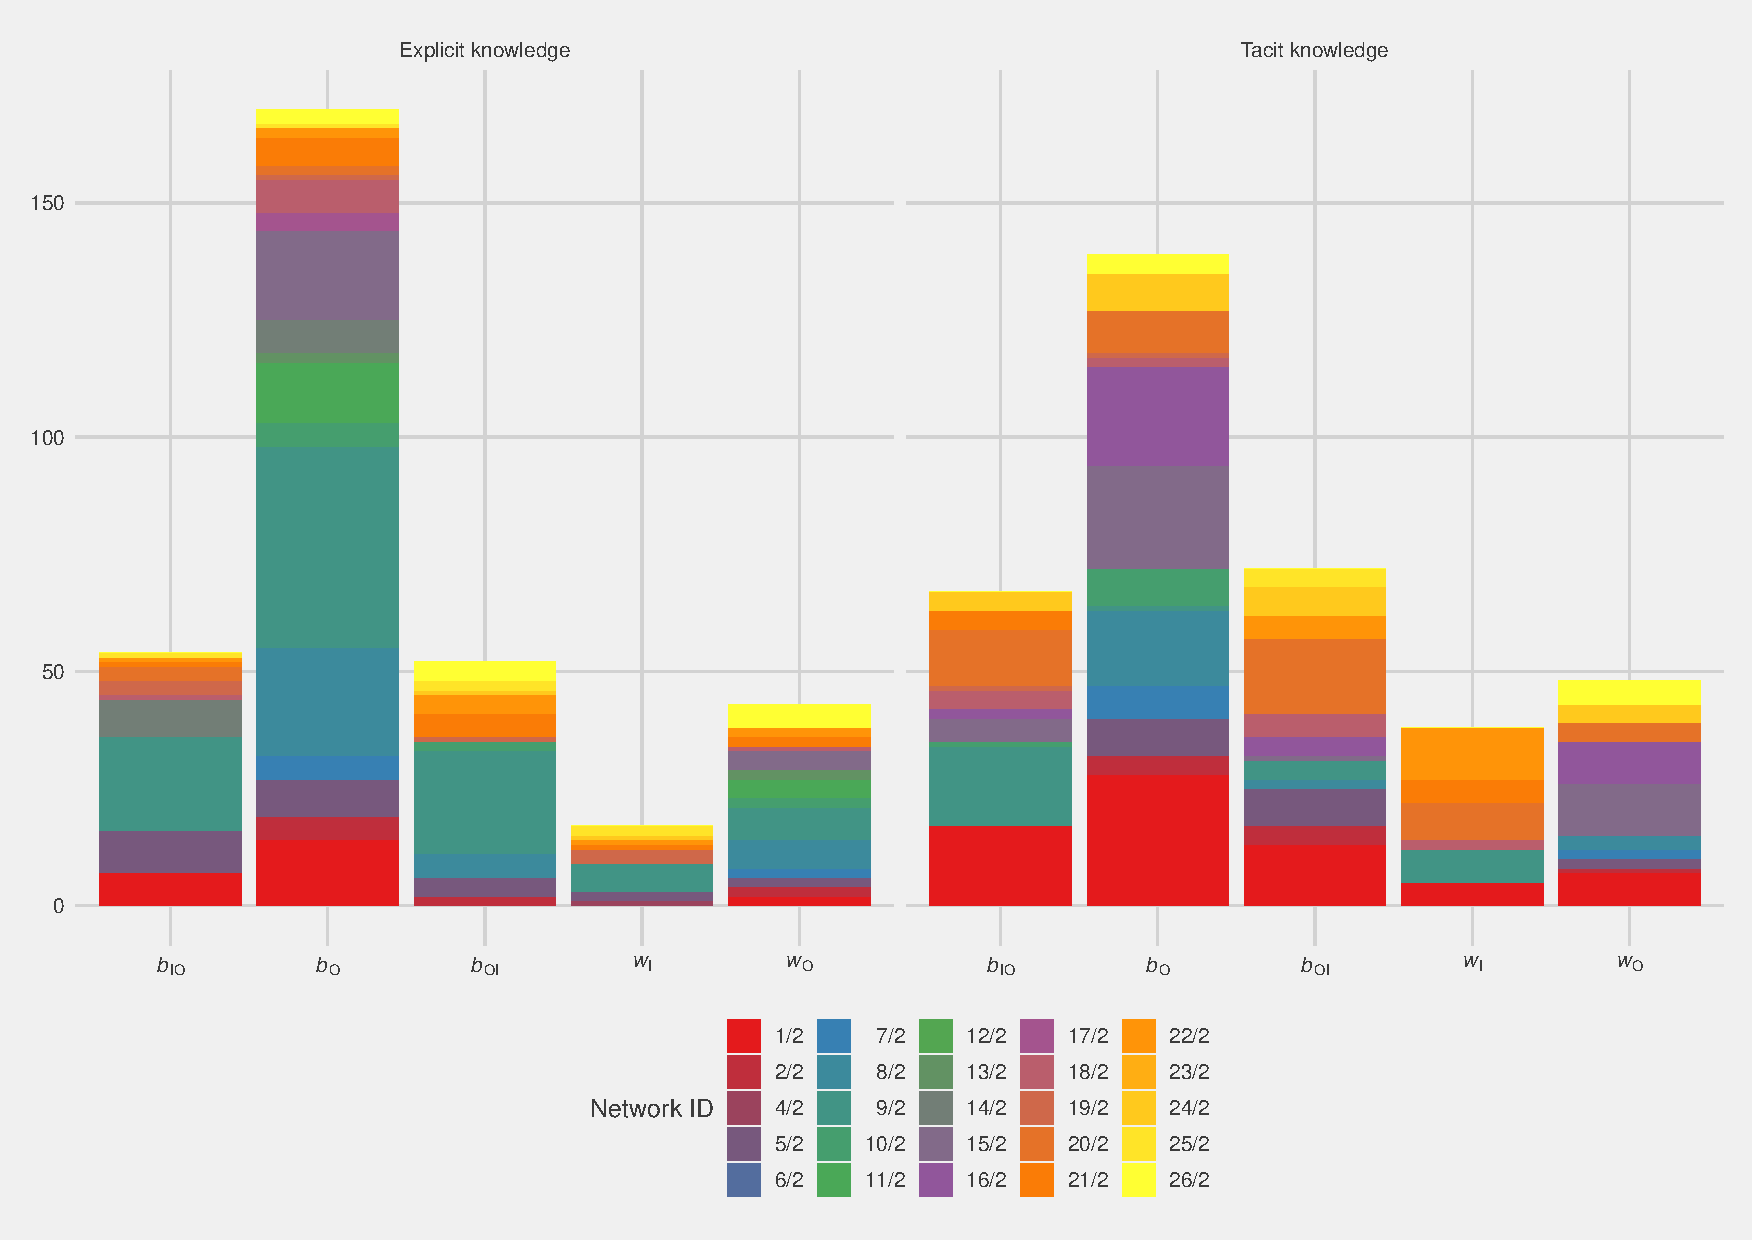
\includegraphics[width = \textwidth]{Images/gf_case2.pdf}
\caption[Breakdown of broker roles by participant in Case 2]{Breakdown of broker roles by participant in Case 2. Note $w_I$ = internal coordinator role, $b_O$ = liaison role, $b_{OI}$ = gatekeeper role, $b_{IO}$ = representative role, and $w_O$ = itinerant broker role.}
\label{fig:gf_c2}
\end{figure}

\subsection{Coding results}

The most used codes in Case 2 refer to trust relations (importance of being open and maintaining good relationships), boundaries (physical distance, foreign cultures, dealing with change), knowledge brokering (representative brokerage), learning (deepen understanding, tapping external know-how), collaborating (breaking new ground, working towards a common goal, showing commitment), and applying knowledge in practice (learn by doing, reflection). Of these, the code \enquote{learn by doing} stands out and goes a long way to explain why tacit knowledge features so strongly in Case 2. As we did with Case 1, we examine the more frequently used codes in context of \citet{loyal2001agency}'s agency model.

\begin{sidewaystable}
\centering
\caption{Top codes in each category: Case 2.}
\label{tab:case_2_codes}
\begin{tabular}{lllc}
\toprule
Category code & Provisional code & Detailed code & References \\ 
\midrule
Innate needs & Motivational forces & Quest for self-efficacy &   5 \\ 
Innate needs & Motivational forces & Desire to do meaningful work &   3 \\
Mechanisms \& structures & Trust relations & Having good relations &  16 \\ 
Mechanisms \& structures & Boundaries & Navigating change &  14 \\ 
Mechanisms \& structures & Trust relations & Having open and honest discussions &  13 \\ 
Mechanisms \& structures & Boundaries & The tyranny of distance &  13 \\ 
Mechanisms \& structures & Boundaries & Dealing with foreign cultures &  12 \\
Action & Learning & Learn by doing &  26 \\ 
Action & Collaborating & Being absolutely committed &  19 \\ 
Action & Doing something novel & Breaking new ground &  19 \\ 
Action & Doing something novel & Profiting from innovation &  17 \\ 
Action & Applying knowledge in practice & Reflecting on what can work &  15 \\ 
\bottomrule
\end{tabular}
\end{sidewaystable}

\subsubsection{Innate needs}

Innate needs did not feature strongly in the responses to interview questions. Both the dairy farmer and the owner of the dealership responsible for installing and servicing the robotic milking technology stated that they really enjoyed working at the cutting edge of technology:

\begin{quote}
\small
\enquote{I enjoy probably from three different angles, I enjoy being on the cutting edge of dairy systems or dairy technology and being at the coalface in terms of developing and driving and creating new systems.} \\
\rightline{\rm --- Participant 1/2}
\end{quote}

\begin{quote}
\small
\enquote{you can call it an ego trip whatever you like, to get involved in something that's cutting edge. And that's what's maintained the motivation.} \\
\rightline{\rm --- Participant 15/2}
\end{quote}

The partnership benefited enormously from the diary farmer's ambition to succeed, which is under-scored by his centrality in the tacit knowledge provider network (Figure \ref{fig:network_case_2}). Some interviewees thought the dairy farmer tied too hard to make things work to prove something either to himself or his industry peers:

\begin{quote}
\small
\enquote{[Name of the dairy farmer] had to prove a point to the industry that the technology could do what we said it was doing.  So he was almost proving, it wasn't for him, it was for the industry, to try and make this a success.} \\
\rightline{\rm --- Participant 9/2}
\end{quote}

\begin{quote}
\small
\enquote{he took it so personally, that if something didn't work it was failure, to his own detriment.} \\
\rightline{\rm --- Participant 15/2}
\end{quote}
 
The dairy farmer may have been driven to satisfy an innate need for competence. While some may think he was too emotionally invested, others saw his determination to succeed as crucial to the success of the venture:

\begin{quote}
\small
\enquote{And I think they recognised that the [dairy farmer was] willing to put the effort in and having seen the effort that went in I wouldn't think there would be too many farms that would be willing to work as hard as [the dairy farmer] did in getting that machine up and running.} \\
\rightline{\rm --- Participant 11/2}
\end{quote}

\subsubsection{Subjective norms}

Subjective norms did not feature strongly in the responses to interview questions. One senior manager from the milking technology provider did remark some of his engineers suffer from \enquote{not-invented-here} syndrome:

\begin{quote}
\small
\enquote{There is a little occasionally not invented here syndrome, so ... which you get from engineers, they think they have the perfect solution and yet there’s an alternative solution outside. So even we have to challenge them at times to think outside the box.} \\
\rightline{\rm --- Participant 18/2}
\end{quote}

However, this never came up as an issue with the other interviewees. No conclusive statements can be made about subjective norms in Case 2. 

\subsubsection{Mechanisms and structures}

Maintaining good relations, physical separation, reconciling different worldviews, and foreign cultures were the key mechanisms and structures affecting knowledge exchanges in Case 2. Investing in relationships was considered vital by some interviewees. Participants tended to be more open and honest with others they had good relations with:

\begin{quote}
\small
\enquote{I don't know that this comes under the trust category, but one thing that influenced a lot of the discussions, often subconsciously was that we were all very mindful that we had relationships that we needed to maintain.} \\
\rightline{\rm --- Participant 8/2}
\end{quote}

\begin{quote}
\small
\enquote{there appears to be strong relationships in this collaboration and I think that's part of all of it because we know each other so well the trust level is very high for the information that's shared.} \\
\rightline{\rm --- Participant 11/2}
\end{quote}

High levels of trust allowed participants to freely exchange ideas and engage in learning: 

\begin{quote}
\small
\enquote{You knew that when you put an idea on the table, people were, you were comfortable with people pulling that idea apart, and people having different opinions, and that’s what it really was all about.} \\
\rightline{\rm --- Participant 8/2}
\end{quote}

\begin{quote}
\small
\enquote{I think it was a really open honest discussion to learn together and capture those learnings. So still today this morning I was participating in another meeting to try to put those learnings together. So I think there was a lot of honest discussions. Each one had their agenda to a certain point, but in those common themes it was about honest discussions to come up with solutions.} \\
\rightline{\rm --- Participant 10/2}
\end{quote}

\begin{quote}
\small
\enquote{I've never been involved with anything like that before where people would openly discuss ideas. And yeah, you'd probably take it for granted as well, same deal; but when you sit back and reflect, there was lots of different skill sets there and people were generally good at sharing their knowledge.} \\
\rightline{\rm --- Participant 15/2}
\end{quote}

The milking technology provider chose to trial their robotic milking technology in a distant country. Doing so was a calculated decision to allow them to experiment with new technology away from the prying eyes of competitors:

\begin{quote}
\small
\enquote{And we agreed some terms of putting an installation in [a relatively remote location], [a relatively remote location] for reasonably obvious reasons from a [technology provider] perspective internationally it was a nice place to do it, it's out of the way, if you mess up it's reasonably easy to handle.} \\
\rightline{\rm --- Participant 18/2}
\end{quote}

Doing a trial in a distant country did create some problems. Resolving technical issues with engineers based in a completely different time-zone was a frustrating experience for the dairy farmer and his local dealer:

\begin{quote}
\small
\enquote{A good example is because we're different time zones and we milk 24 hours a day then if we have a problem in the middle of the day at our place it's the middle of the night in [the Scandinavian country where the robotics engineers are based] and in the very early years we were given phone numbers to people to communicate because it's cutting edge and nobody could deal with it locally.} \\
\rightline{\rm --- Participant 1/2}
\end{quote}

\begin{quote}
\small
\enquote{but it's not much fun the time difference, when you have got an issue, it always happened on a Friday night or a Saturday night, it's just Murphy. So, to actually get a hold of people on the other side of the world that you need to get hold of, that was a challenge at times. To get that expertise and knowledge that you require.} \\
\rightline{\rm --- Participant 15/2}
\end{quote}

Apart from the frustration of having to work across different time-zones, physical separation was not a significant barrier to tacit knowledge sharing (Table \ref{tab:ergm_1}). The milking technology was willing to send robotics engineers across the world to witness things on the dairy farm firsthand:

\begin{quote}
\small
\enquote{often we'd say \enquote{listen you've got to send these engineers down here} because we're experiencing things that are creating fatigue in the system and wear and tear that we don't see anywhere else with the older technology we have so we really need to get on top of it.} \\
\rightline{\rm --- Participant 9/2}
\end{quote}

Linguistic barriers did cause some issues. Both the Scandinavian and Australian participants would say things to each other in English that were often interpreted too literally instead of figuratively (people from different cultures could not comprehend particular turns of phrases). Misinterpreting what is said makes the already difficult task of communicating tacit knowledge that much harder:

\begin{quote}
\small
\enquote{Well talking to a [Scandinavian] person, they may speak pretty good English, they don't understand Australian real well, and probably vice versa. So them actually interpreting what you were saying, whether it was from a technical aspect or whatever. That can be frustrating at times. So you might have been telling them something and they would think it was completely opposite.} \\
\rightline{\rm --- Participant 15/2}
\end{quote}

\begin{quote}
\small
\enquote{I've had to step in on a number of occasions [when dealing with the main head-office] and it's probably the cultural side and sitting down with the likes of [the diary farmer and his father] and trying to explain to them what is a .. when [a Scandinavian person] says yes, they actually mean no.} \\
\rightline{\rm --- Participant 18/2}
\end{quote}

\begin{quote}
\small
\enquote{I will say that a word that people like to use is \enquote{no worries}, but even if you hear that word it might not be that there is no worries.  There are something behind that word that meaning that you have to learn how to read that when you get that answer.} \\
\rightline{\rm --- Participant 24/2}
\end{quote}

Implementing a very novel farm system to support voluntary milking required people to see things in a  different light. The dairy farmer had to change his approach to cow nutrition because how you move cows through the system is done by managing their grazing habits. He was used to using supplements, which did not lend itself to voluntary milking. He had to adjust his way of thinking:

\begin{quote}
\small
\enquote{My focus is always on trying to maximise the use of pasture and so when I first went there I'm confronted with a farm that's feeding enormous amounts of supplements and has paddocks that are vastly under-utilised and I found that difficult because I want more cows to eat more grass whereas he was more concerned about maintaining a higher production ... [the dairy farmer's] philosophy compared to mine is a boundary and we had to work around it and I think we did that quite successfully.} \\
\rightline{\rm --- Participant 11/2}
\end{quote}

The engineers from the milking technology company were not used to pasture-based farm systems. They were more familiar with the practice of housing rather docile dairy cows in barns, which influenced how they designed their technology. Dairy cows in pasture-based systems behave quite differently. Their milking robots struggled to cope with unfamiliar cow behaviour and it took a while for the engineers to adapt to a different reality:

\begin{quote}
\small
\enquote{I would also have to provide animal farm system knowledge back to the technical guys because they had no idea. To them a cow is four legs and four teats and I've got to put a robot, get a robot to cup those cows.  So I'd have to give them a bit of behaviour knowledge and say, tell them why cows weren't coming at certain times of the day because cows do what cows do.} \\
\rightline{\rm --- Participant 9/2}
\end{quote}

\begin{quote}
\small
\enquote{one main thing is that batch milking is the way we are doing it overseas, to say, or Europe and down under we’re trying to voluntary cow traffic.} \\
\rightline{\rm --- Participant 24/2}
\end{quote}

\begin{quote}
\small
\enquote{I can remember one bloke coming over, and he'd spent a day just looking for cows, and why would you put them out on the grass because they don't do that over there. So they were just fascinated about how we were trying to get the system to run: why would you do that, why wouldn't you just put them in a shed and house them?} \\
\rightline{\rm --- Participant 15/2}
\end{quote}

\subsubsection{Actions}

Actions that stand out include learning from experience, showing commitment, breaking new ground, working towards a common goal, striving for a profitable outcome and reflecting on what does or does not work. Learning featured strongly in this case. It was achieved by experimenting with different approaches to see what does or does not work:

\begin{quote}
\small
\enquote{I know they tried different things. At one stage they had a forage crop that they were trying to get the cows to eat, and the cows just stopped trafficking to the crop, because they didn't like it, because it had become too mature. So there were hurdles along the way like that, that we all learned a lot from.} \\
\rightline{\rm --- Participant 8/2}
\end{quote}

Much of the learning was forced onto participants. To make things work participants had no choice but to learn things on the fly:

\begin{quote}
\small
\enquote{We were thrown into a herd management software and given zero formal training from [the technology provider]. All of that was self-taught and if it hadn't been a 24 year old Gen Y'er I doubt that person would have coped unless they were an absolute computer boffin. It is a very IT sensitive type of technology. There was an awful lot of self-teaching.} \\
\rightline{\rm --- Participant 1/2}
\end{quote}

\begin{quote}
\small
\enquote{I saw [being a partner] as an opportunity to fast track our learning, and I reckon in two years we got ten years' worth of experience. Now you can't put a value on that. But since then, we've done three other robot farms, just conventional robots, and we've had no problems because of that knowledge base that we've gained.} \\
\rightline{\rm --- Participant 15/2}
\end{quote}

One thing that stands out in Case 2 is the level of commitment and passion shown by all the partners. Everyone was strongly committed to delivering a successful outcome:

\begin{quote}
\small
\enquote{I don't think a lot of the [partners] understood at a farm level how much time was consumed in actually making this work at a practical level. A lot of the [milking technology company employees] could log off and go home where we were left to run and manage it and for three years I was doing close to 100 hours a week. It's a colossal commitment.} \\
\rightline{\rm --- Participant 1/2}
\end{quote}

\begin{quote}
\small
\enquote{It just showed the level of passion that people had, that they didn't just turn up for the meeting because that's what they were paid to do or whatever. They actually really cared.} \\
\rightline{\rm --- Participant 8/2}
\end{quote}

\begin{quote}
\small
\enquote{if you say to [the dairy farmer] \enquote{Can you do this?} he'll do it. Sometimes \enquote{Can I have it tomorrow?} it might come the next day but it's – he'll get it done for you. And he’s fantastic like that.  I mean [the lead dairy researcher is] also great like that.} \\
\rightline{\rm --- Participant 9/2}
\end{quote}

\begin{quote}
\small
\enquote{And I think they recognised that the [the dairy farmer was] willing to put the effort in and having seen the effort that went in I wouldn't think there would be too many farms that would be willing to work as hard as [the dairy farmer] did in getting that machine up and running.} \\
\rightline{\rm --- Participant 11/2}
\end{quote}

While nobody doubts the level of commitment shown by the farmer, the milking technology provider also showed commitment by investing a lot more capital in their commercial pilot than what they had originally had planned to do:

\begin{quote}
\small
\enquote{But a lot of it at the end of the day was [the milking technology provider] had to step up with capital and I think at the end of the day there was a lot more capital that went into this than what [the provider] was ever expecting.} \\
\rightline{\rm --- Participant 9/2}
\end{quote}

Although the dairy farmer appears to have been motivated to satisfy an innate need for competence, much of the commitment can be attributed to a shared desire to revolutionise the dairy industry. The dairy farmer felt that traditional dairy farming was a difficult and lonely profession. He wanted to do something to make dairy farming more appealing and fulfilling:

\begin{quote}
\small
\enquote{I think in our situation, innovation is trying to find a better, more profitable, more socially acceptable method of dairy farming.} \\
\rightline{\rm --- Participant 1/2}
\end{quote}

The dairy researchers enjoyed seeing their ideas finally realised in a commercial dairy operation:

\begin{quote}
\small
\enquote{for me it was a nice way to finish up what had been a fairly long process of co-development and testing, and working with a prototype and to actually see it being implemented on farm, it was a very rewarding thing.} \\
\rightline{\rm --- Participant 8/2}
\end{quote}

\begin{quote}
\small
\enquote{I like the fact that this has never been done anywhere in the world, and we were doing ground proving knowledge that had never done before, and asking questions and finding solutions for problems that nobody had faced before. So it was quite stimulating from that point of view.} \\
\rightline{\rm --- Participant 10/2}
\end{quote}

For the milking technology provider, the goal was to prove a farming system that would help them sustain their competitive advantage. 

\begin{quote}
\small
\enquote{So if we get this technology along with grazing systems and maybe not voluntary cow traffic there, but certainly with a grazing capability, then we set ourselves up to be stepping ahead of our competitors in this particular area.  We are still number one around the world as far as the market position, although there are lots of what we call \enquote{grey competitors} which are smaller local players and when you had, shall we call it, conventional milking which twenty years ago was, shall we say, reasonably advanced as we brought more electronics into the farming operation, everybody quickly catches up and for them to compete with us on a different platform means that they have to really step up from an engineering perspective to be able to compete.} \\
\rightline{\rm --- Participant 18/2}
\end{quote}


















 





\subsubsection{Synopsis}



\subsection{Case 3}

\subsubsection{Semi-structured interviews}

Of the 40 people who participated in Case 3, only seven were interviewed (Table \ref{tab:interview}. The plan was to interview double this number of people, but resentment stemming from unmet or unrealistic expectations, telecommunication problems, and foreign language issues frustrated efforts. Three of the seven interviews were face-to-face. Interviews took between 30 and 90 minutes to complete (the average interview duration was 53 minutes). \medskip

Table \ref{tab:sentiment_case_3} shows the overall sentiment expressed by interviewees in their responses to questions. Although two interviewees came across quite positive (Participants 10/3 and 16/3), the overall sentiment is less positive than the other two cases. Figure \ref{fig:bigram_case_3} highlights what interviewees mainly spoke about. Topics that stand out include \enquote{global initiative}, \enquote{honey bee[s]}, \enquote{bee health}, \enquote{stingless bees}, and \enquote{data format}.

\subsubsection{Recap of network analysis}

Results from the social network analysis show that explicit knowledge provider ties outnumber tacit knowledge provider ties (Figure \ref{fig:network_case_3}). As this case is about providing an innovative web-based data analysis platform, we expect explicit knowledge to feature strongly. However, working with different bee species does require much know-how or tacit knowledge. \medskip

The ERGM results show that a small number of central actors provide most of the tacit knowledge. Many tacit and explicit knowledge providers also operate as brokers. Contrary to expectations, tacit knowledge providers tend to be extrinsically motivated (previous studies show a strong relationship between intrinsic motivation and tacit knowledge sharing). As with the other two cases, receivers of tacit knowledge tend to be autonomously motivated. Providers of tacit knowledge do not identify strongly with their workgroup. We also see evidence of mutual sharing of tacit knowledge across organisational boundaries, a sign of good collaboration. Participants tend to share their know-how with others they trust. There is evidence of age homophily in the explicit knowledge provider network (people tend to share explicit knowledge with others of a similar age). More experienced people are less likely to share explicit knowledge. Explicit knowledge tends to be directed to superiors and is more likely to be shared with others in close proximity. \medskip

Brokerage features strongly in Case 3. Because this open innovation partnership was at a very early stage at data collection, participants were still getting to know each other. We expect brokers would be essential to help establish the partnership. The ERGM analysis of broker roles shows that the gatekeeper and representative roles are over-represented, and the itinerant broker role is under-represented in the tacit knowledge provider network. The liaison broker role is under-represented in the explicit knowledge provider network (Table \ref{tab:ergm_3}). Looking at the raw broker counts presented in Figure \ref{fig:gf_c3}, Participant 10/3 dominates all but the itinerant broker roles. Participant 10/3 is the most central actor in both the explicit and tacit knowledge networks.

\begin{figure}
\centering
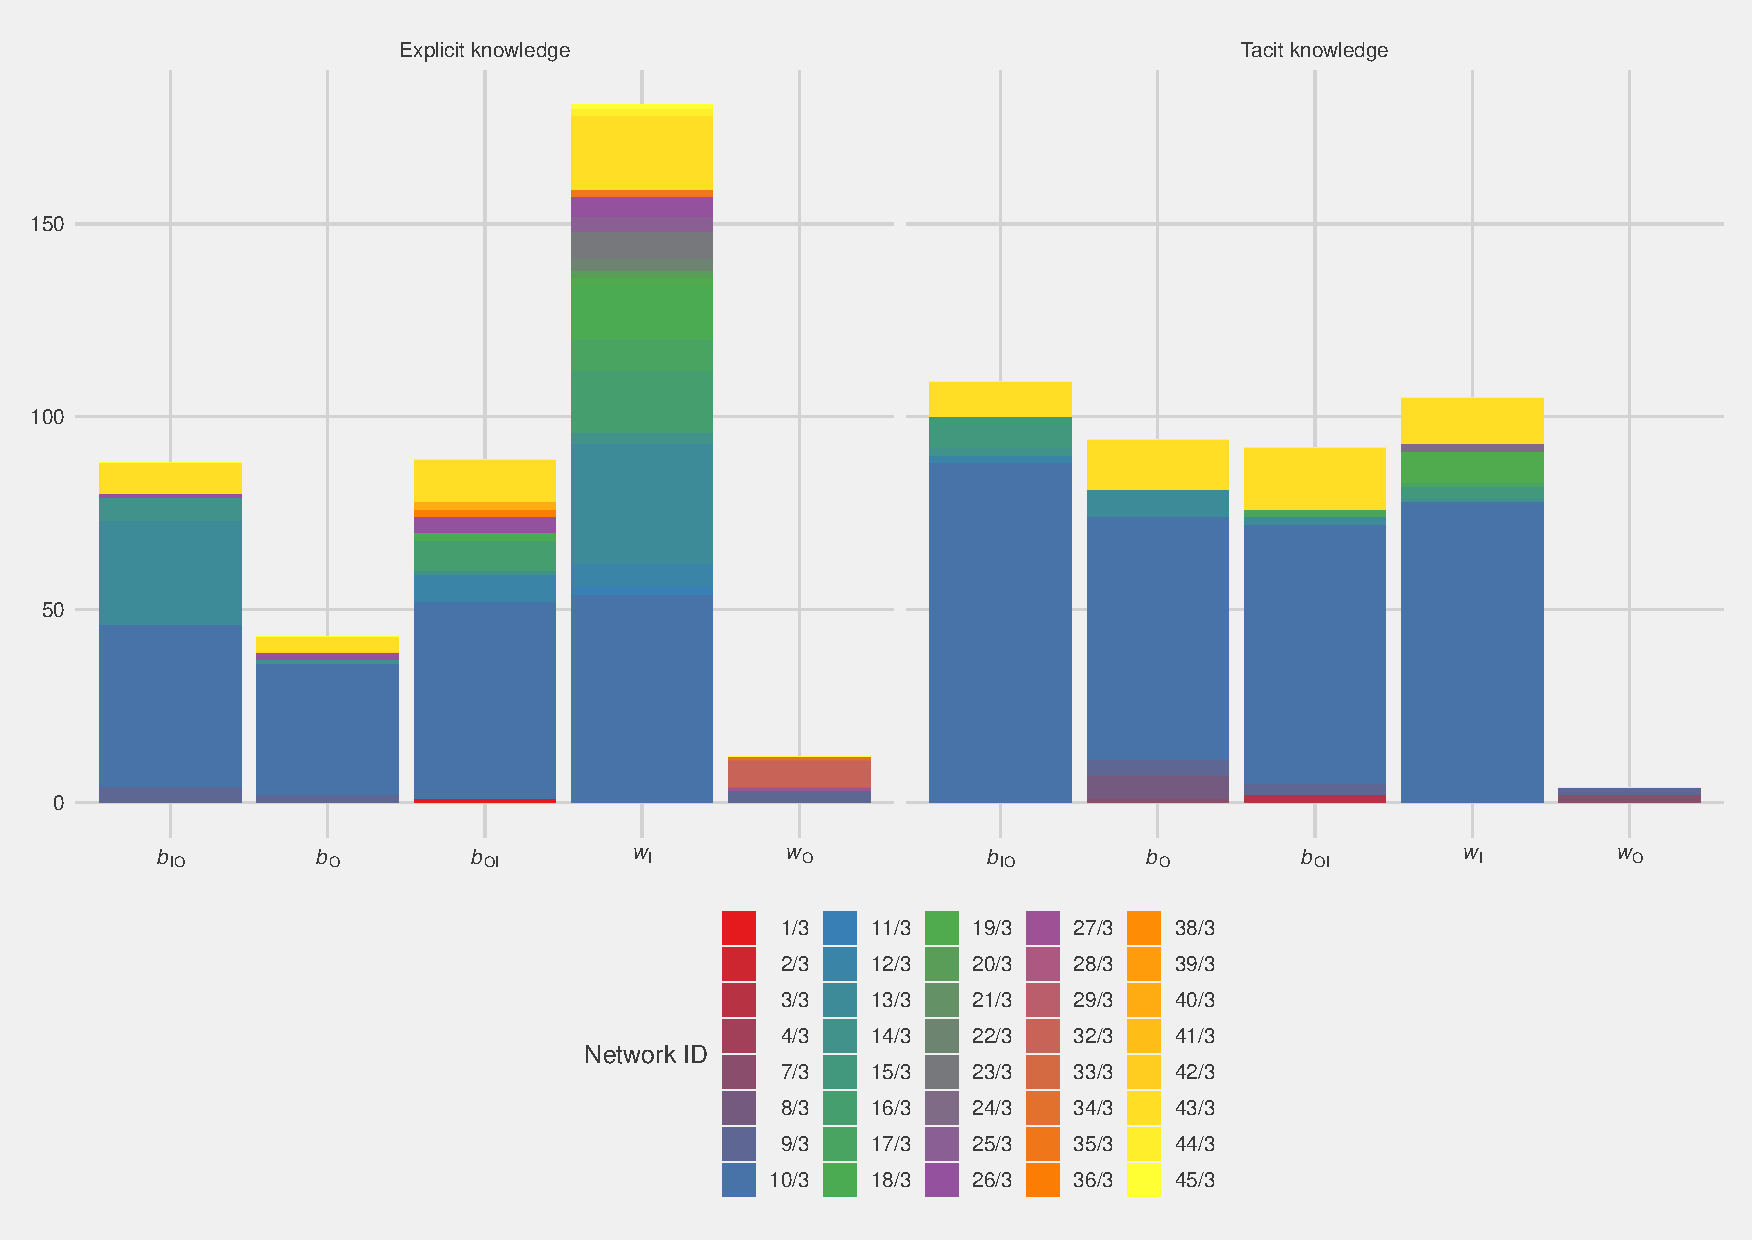
\includegraphics[width = \textwidth]{Images/gf_case3.pdf}
\caption[Breakdown of broker roles by participant in Case 3]{Breakdown of broker roles by participant in Case 3. Note $w_I$ = internal coordinator role, $b_O$ = liaison role, $b_{OI}$ = gatekeeper role, $b_{IO}$ = representative role, and $w_O$ = itinerant broker role. As with the other two cases, the itinerant broker role hardly features. Participant 10/3 stands out as a dominant broker, especially in the tacit knowledge network.}
\label{fig:gf_c3}
\end{figure}

\subsection{Coding results}

Table \ref{tab:case_3_codes} lists the most referenced codes in each category for Case 3. As with the other cases, \enquote{innate needs} and \enquote{subjective norms} did not feature strongly in responses to interview questions. Unrealistic expectations, poor communication, cultural boundaries, funding constraints, and organisational boundaries are the main social mechanisms and/or structures moderating knowledge exchanges. Actions revolve around people acting in their self-interest, a strong desire to codify knowledge, working towards a common goal, and engaging in reflective practice. \medskip

\begin{sidewaystable}
\centering
\caption{Top codes in each category: Case 3.}
\label{tab:case_3_codes}
\begin{tabular}{lllc}
\toprule
Category code & Provisional code & Detailed code & References \\ 
\midrule
Innate needs & Motivational forces & Quest for self-efficacy &   3 \\ 
Subjective norms & Expressing a particular worldview & Maintaining a narrow perspective &   5 \\ 
Mechanisms \& structures & Boundaries & Poor communication &  19 \\ 
Mechanisms \& structures & Boundaries & Dealing with foreign cultures &  12 \\ 
Mechanisms \& structures & Boundaries & Limited resources &   7 \\ 
Mechanisms \& structures & Boundaries & Organisational boundaries &   7 \\ 
Mechanisms \& structures & Trust relations & Having open and honest discussions &   6 \\ 
Action & Collaborating & Managing expectations &  28 \\ 
Action & Collaborating & Acting in self-interest &  27 \\ 
Action & Learning & Codifying knowledge &  10 \\ 
Action & Collaborating & Working towards a common goal &   9 \\ 
Action & Applying knowledge in practice & Reflecting on what can work &   8 \\ 
\bottomrule
\end{tabular}
\end{sidewaystable}

\subsubsection{Innate needs}

As with the other two cases, the network analysis shows receivers of tacit knowledge tend to be autonomously motivated. For some interviewees, the quest for self-efficacy was a big personal motivator. Being involved in this partnership presented them with an opportunity to master new technology: 

\begin{quote}
\small
\enquote{I love to learn new things and this is the good thing from the project for sure.} \\
\rightline{\rm --- Participant 9/3}
\end{quote}

\begin{quote}
\small
\enquote{After a very long breakaway from computer systems engineering I'm back working with embedded systems. So this is actually beneficial because it's a change in pace away from just pure software engineering and web applications, and it diversifies and expands my skill-set.} \\
\rightline{\rm --- Participant 16/3}
\end{quote}

\begin{quote}
\small
\enquote{With this project I have a more intimate contact with a different kind of technology and the [importance] for me is that I can adapt [the] technology in my ... for my [research interest].} \\
\rightline{\rm --- Participant 39/3}
\end{quote}

\subsubsection{Subjective norms}

A couple of the interviewees believe that scientists are either too focused on their area of expertise or risk-averse. They think scientists feel pressure to compete with others in their field. They are reluctant to take risks as their ability to attract funding depends on their track record of delivering successful research outcomes:

\begin{quote}
\small
\enquote{Scientists are competing for small discoveries, and trying to publish a paper that shows a small conclusion about a specific topic. And doing that of course, they end up losing the big picture of what they can achieve if they join forces. And I think this is what is missing.} \\
\rightline{\rm --- Participant 10/3}
\end{quote}

\begin{quote}
\small
\enquote{We largely see in science these days small incremental improvements and that's largely because the corporate and scientific community in the western societies now has become very risk averse. So people are ... their funding is tied to success, so they're reluctant to take big risks to think outside the box to try something completely different, and so they just do little incremental improvements on what's already known.} \\
\rightline{\rm --- Participant 16/3}
\end{quote}

 These statements point to some tension within the partnership. It seems the partnership was struggling to gain traction because not all the participating scientists were willing to try something radically different or expand their scope of research.

\subsubsection{Social mechanisms \& structures}

The main social mechanisms affecting knowledge flows included poor communication, language barriers, limited funding, organisational boundaries, and trust issues. Although the network analysis indicates geography was a factor for explicit knowledge exchanges, it seems geography was a major factor affecting communication. The reliance on email communication was considered an issue:

\begin{quote}
\small
\enquote{Communication also, it's one of the, it brings a lot of boundaries as well, because we are so inefficient in the way we write, email is not necessarily the best tool for us to exchange information, so we need to talk, and that changes completely, because visual communication helps so much. You need to be aware that emails can be misunderstood, there are many other aspects. And there are the acquired aspects of the barrier. Somebody's not talking, but the body language is telling you so much, or the science tells you a lot, the person just went quiet, what's going on? So there is something going on there.} \\
\rightline{\rm --- Participant 10/3}
\end{quote}

The partnership relied on a \enquote{hub-and-spoke} management model. All communication was directed through the national research agency. This mean that partners were not really aware of what others were doing:

\begin{quote}
\small
\enquote{it appears that the group here at [the national research agency] are acting as a central hub.  So it’s basically a hub and spoke model, or a star model – however you want to describe it – we're the hub, and each collaborator is a node at the end of a spoke.  And there is ... between Mexico and Brazil I think there might be some cross-communication, but largely information comes back to us and then gets disseminated out to people who might need it.  So it's ... we've become like the centralised information broker.} \\
\rightline{\rm --- Participant 16/3}
\end{quote}

\begin{quote}
\small
\enquote{I don't know that any of it is deliberate, it's just that everybody's got particular instructions of what they're meant to be doing, and some of them aren't aware of the background, or aren't aware of who else was operating in the space. And so, yeah, there was just some unusual things that have been happening.} \\
\rightline{\rm --- Participant 22/3}
\end{quote}

For a hub-and-spoke model to work well requires the hub to be very effective at disseminating information. Unfortunately, the national research agency was not always an effective communicator. Failing to follow-up on email communication was an issue:

\begin{quote}
\small
\enquote{Between the two of our groups, when we have an issue we send an email, maybe it gets a reply, maybe it doesn't. And when [the national research agency] needs something they send an email, maybe it gets a reply, maybe it doesn't. There's  no ongoing conversation really happening.} \\
\rightline{\rm --- Participant 41/3}
\end{quote}

Language was also a significant barrier to effective communication. Not all the participants felt comfortable conversing in English and were less open as a consequence:

\begin{quote}
\small
\enquote{For sure, for sure it is because all Portuguese-speaking people are involved and not everyone here has good English and they are afraid, they want to but they don't know how to expose and even to understand the other opinions and contributions from English-speaking people.} \\
\rightline{\rm --- Participant 9/3}
\end{quote}

Support for the global partnership was patchy within the national research agency. Although the initiative generated much media attention for the agency, it was reluctant to support ongoing efforts. The team driving the initiative ran out of funding to progress things: 

\begin{quote}
\small
\enquote{Well we haven't got a budget anymore.  We haven't got any money, so it makes it very difficult to progress relationships with kits, give ... apart from the fact they're not developed yet. But even if they were we haven't got any money, so we have no operational money left.} \\
\rightline{\rm --- Participant 13/3}
\end{quote}

The agency is expected to source a significant portion of its revenue through externally-funded contacts. One senior manager questioned why anybody would want to invest in this global initiative:

\begin{quote}
\small
\enquote{if the [global partnership] is going to grow to the scale that [the main protagonist] has ambition for, there's got to be significant flows of cash somewhere, or resources. And so you've got to be able to interest someone to want to invest and they're either going to be a ... do it for philanthropic purposes or they're going to want to see a commercial return.} \\
\rightline{\rm --- Participant 22/3}
\end{quote}
 
Those responsible for business development within the agency did not seem particularly motivated to secure additional funding for this initiative. Perhaps this is because they are rewarded for landing big external contacts and did not see much chance of securing substantial funding:

\begin{quote}
\small
\enquote{I don't understand why [the agency business unit] were even involved, and their business development person, and two years, talked a lot but did nothing. And now they've gone and we were meant to be assigned another one, and I haven't seen any progress out of that.} \\
\rightline{\rm --- Participant 13/3}
\end{quote}
 
The lack of funding meant that progress was frustratingly slow. Unmet expectations gave rise to resentment that ultimately hampered knowledge sharing between partners: 

\begin{quote}
\small
\enquote{I think there could be a lot more progress, but I think relationships and finance, and all of that is hampering any progress. I think if there was more progress there would be more knowledge sharing, but everyone's still just trying to get off the ground.} \\
\rightline{\rm --- Participant 13/3}
\end{quote}

\subsubsection{Actions}

Failure to manage expectations, people acting out of self-interest, efforts to codify knowledge, trying to get people to work towards a common goal, and reflecting on what works are key actions that influenced the way the global partnership operated. The partnership was launched with great fanfare and attracted global media attention. Unfortunately, the technology for tracking bee movements in and out of hives was still being developed. Partners signed on to the initiative expecting the technology to work out the box. Teething problems caused some participants to become disillusioned:

\begin{quote}
\small
\enquote{I'm a little worried because I went for this one year ago and we didn't have so far an example of the final thing working. We just say [to our principals] the equipment [is capable] but we need something ready, working, at the final stage, as soon as possible.} \\
\rightline{\rm --- Participant 9/3}
\end{quote}

\begin{quote}
\small
\enquote{I think the promise always was that the sensors and the technology was all well developed and straightforward and all you needed was to pick up the sensors and apply them to your bees and do a bit of programming and everything would work.} \\
\rightline{\rm --- Participant 22/3}
\end{quote}

It appears many of the participants did not fully appreciate the technical challenge of building a cloud-based data management system with limited resources:

\begin{quote}
\small
\enquote{I think that there's a perception amongst the scientists that the technical stuff should just be simple because it's not science, right? It's just engineering and anyone can do that and crank the handle, and they don't really understand the challenges involved in building the technical solution that they're looking for.} \\
\rightline{\rm --- Participant 16/3}
\end{quote}

Expectations may have been more realistic had there been more effective communication. The hub-and-spoke model did not allow partners to easily share their experience of getting the technology to work. Disappointment in the technology gave rise to concern about possible reputational damage to the national research agency. This concern may explain why internal support for the global partnership did not eventuate:

\begin{quote}
\small
\enquote{I was getting concerned about our international profile and whether we were going to be ... I was just worried about all these groups overseas who might know honey bees but don't know technology too much and whether they're going to be pissed off by the [agency] product.} \\
\rightline{\rm --- Participant 22/3}
\end{quote}

Even though some partners were disappointed the technology did not meet expectations, they did not have to pay for technology starter kits and were motivated to join the partnership to further their own research interests:

\begin{quote}
\small
\enquote{It came from scientists around the world and from bee keepers, asking to have access to the technology that we have developed at [the national research agency]. They became aware of that because of a media campaign we have done, and a result of that huge exposure from the media, they became aware of the research, and they started looking at how can they work with us, because they have a number of questions they would like to answer using this technology.} \\
\rightline{\rm --- Participant 10/3}
\end{quote}

\begin{quote}
\small
\enquote{I guess we benefit in the sense that we get access to technology that would have been very difficult to access earlier and I guess that's true of anybody who’s partnering with [the national research agency]. It's very hard to get, even just to buy the RFID chips, it's quite difficult, if you're buying less than one million of them. So it works from a logistics sense to have everybody working together on that front. And then [the agency] obviously benefits in the sense that it gets the data from everybody who's working in the [partnership].} \\
\rightline{\rm --- Participant 41/3}
\end{quote}
 
One of the goals of the partnership was to develop a standardised data repository. Everybody would provide or access data in a standard format. Because scientists wanted to collect data to answer specific research questions, agreeing to a standardised way of collecting and managing data proved quite challenging. Each partner wanted a custom set up that suited their way of thinking, which was at odds with the idea of performing big data analytics on a common data set. Unlike the other two cases, there was no proper commitment to a common objective:

\begin{quote}
\small
\enquote{The original idea was that everyone would do the same experiments using the same protocols with the same equipment so that everything would be standardised and we could do comparative analysis. It became apparent very quickly that that wasn't going to be the way things worked, because each partner has strong opinions on what science they would like to do.} \\
\rightline{\rm --- Participant 16/3}
\end{quote}

Partners were also reluctant to share their data with others, fearing that others would publish their results before them. Essentially, the partners were wary of each other and not particularly open or trusting:

\begin{quote}
\small
\enquote{And so there's some reluctance to share data because someone might just take your data and publish it before you. And I guess that's a trust issue, and that takes time for them to decide that that's not going to happen in this case.} \\
\rightline{\rm --- Participant 16/3}
\end{quote}

To facilitate the sharing of know-how, the team driving the global partnership set up a project wiki to allow participants to capture their learnings. The idea was that partners would update the wiki, but it seems not everyone bought into this idea. One of the team members driving the initiative wrote up most of the experimental setups used by partners. Partners kept their know-how confined to their group or preferred to describe experimental setups in their publications:

\begin{quote}
\small
\enquote{I'm a person who likes to formalise and document stuff, and the reason behind that is if I can formalise and document stuff, then that becomes a resource for those people and I can make that available to them and they can have a look at it any time that they want ... so I've done all the experimental set up documentation, this experiment was run from this date to this date, it used these pieces of equipment, they were configured in this way, they were placed in these locations, those sorts of things.} \\
\rightline{\rm --- Participant 16/3}
\end{quote}

\begin{quote}
\small
\enquote{If you really have something that could help other people in the future we try to describe the protocols in publications.} \\
\rightline{\rm --- Participant 9/3}
\end{quote}

\begin{quote}
\small
\enquote{Generally [knowledge sharing is] practised within our group that any work that we do, we keep details and instructions so somebody else could do it. And so that helps quite a lot with sharing the ... sharing knowledge within our group.} \\
\rightline{\rm --- Participant 41/3}
\end{quote}

At the end of the day, the person who championed the wiki realised its was not the most effective tool for knowledge sharing. He felt it did not facilitate open discussion or idea generation and was keen to try something different:

\begin{quote}
\small
\enquote{I'm of the opinion that the current wiki approach is not conducive to knowledge sharing ... it's not conducive to knowledge sharing, it’s too static and it's ... you've got discrete little bundles of knowledge that are spread across multiple pages within the wiki: it doesn't facilitate discussion. I guess we could set it up to run a forum which is one of my suggestions, I think there should be an open forum between the collaborators where they feel ... where they don't feel intimidated to ask any questions.} \\
\rightline{\rm --- Participant 41/3}
\end{quote}

The senior manager was critical of the leadership of the global partnership. He thought the team driving the initiative had not succeeded in setting out a common vision that everybody could aspire to:

\begin{quote}
\small
\enquote{if we're going to have something that we want to call a \enquote{global initiative}, we'd have to ensure that everybody is on-board with a common vision from the start, and I think we have to seriously look at the leadership skills of those that we expect to lead. So I think we could do better there.} \\
\rightline{\rm --- Participant 22/3}
\end{quote}

Despite the tension stemming from unmet expectations, poor communication, vested interests, and issues around leadership, a lot of learning took place. Partners were exposed to new technology and had to figure out how to tag various bee species in more efficient ways. The team building the data repository gained insight into what bee researchers were most interested in, which helped improve the overall system design:

\begin{quote}
\small
\enquote{It could be the entomologists, or the other scientists, can be the people developing the hardware, it's the same approach with either, it's like well we've discussed this, we know that we need to do this. In order to do that I need the following information because I need this kind of detail, and I'll provide answers, and then from there I'll go OK, given that, well then there’s a whole range of implicit assumptions in that which are these, these, these, and these. Are they correct?  These are the correct assumptions or is there something I've missed here. Essentially, I'm trying to elicit detail without forcing them to sit down and list it all out explicitly.} \\
\rightline{\rm --- Participant 16/3}
\end{quote}

\subsection{Synopis}

Case 3 was struggling to get off the ground. Despite being launched with great fanfare and attracting interest from bee researchers worldwide, it was not well resourced. The hub-and-spoke management model meant the national research agency operated as a significant gatekeeper. Not only did this limit tacit knowledge exchanges, but it also did not help build trust among partners. Disseminating information via email and the wiki proved to be problematic. Language barriers did not help communication either. Partners put their research interests ahead of the global partnership. They were quick to take advantage of gaining access to free technology were also quick to complain it did not work out the box. Organisational politics also got in the way, judging from the patchy support within the national research agency. Nonetheless, participants did learn how to use the new technology and probably developed a greater appreciation of the technical difficulty of setting up a centralised data repository. The team behind the global partnership were probably a bit naive. They should have spent more time developing a shared vision for the global partnership and thought more about the social challenges of running a global open innovation partnership.

\section{Summary}


Table \ref{tab:filtered_codes} highlights subtle but important differences between the qualitative codes for Cases 1 to 3.

\begin{landscape}
\footnotesize
\singlespacing

\begin{longtable}[c]{lllrrr}
\caption[Breakdown of codes by case]{Breakdown of code references by case. Codes referenced two or less times in a case are discounted in our analysis. The breakdown of codes allows one to compare and contrast cases.\label{tab:filtered_codes}} \\
\toprule
Category code & Provisional code & Detailed code & Case 1 & Case 2 & Case 3 \\
\endfirsthead

\multicolumn{6}{c}{Table \ref{tab:filtered_codes} continued from previous page.}\\
\toprule
Category code & Provisional code & Detailed code & Case 1 & Case 2 & Case 3 \\
\midrule
\endhead

\bottomrule \\
\endfoot

\bottomrule
\endlastfoot

\midrule
Action & Applying knowledge in practice & Dealing with complexity & 10 & 3 & 7 \\ 
Action & Applying knowledge in practice & Importance of face-to-face interactions & 9 & $\leq$ 2 & 5 \\ 
Action & Applying knowledge in practice & Improving practices & 30 & 6 & $\leq$ 2 \\ 
Action & Applying knowledge in practice & Integrated thinking & $\leq$ 2 & 4 & 3 \\ 
Action & Applying knowledge in practice & Reflecting on what can work & 3 & 15 & 8 \\ 
Action & Applying knowledge in practice & Relying on tacit knowledge & $\leq$ 2 & $\leq$ 2 & 5 \\ 
Action & Applying knowledge in practice & Using data to guide decisions & 9 & $\leq$ 2 & $\leq$ 2 \\ 
Action & Applying knowledge in practice & Working in different contexts & $\leq$ 2 & 3 & 7 \\ 
Action & Brokering exchanges & Company representative & $\leq$ 2 & 14 & $\leq$ 2 \\ 
Action & Brokering exchanges & Excluding others & $\leq$ 2 & $\leq$ 2 & 6 \\ 
Action & Brokering exchanges & Gatekeeping & 11 & $\leq$ 2 & 4 \\ 
Action & Brokering exchanges & Liaison brokerage & 17 & $\leq$ 2 & $\leq$ 2 \\ 
Action & Collaborating & Acting in self-interest & 4 & $\leq$ 2 & 27 \\ 
Action & Collaborating & Being absolutely commited & $\leq$ 2 & 19 & $\leq$ 2 \\ 
Action & Collaborating & Embracing multidisciplinarity & 3 & 3 & 4 \\ 
Action & Collaborating & Ensuring everyone benefits & $\leq$ 2 & $\leq$ 2 & 5 \\ 
Action & Collaborating & Managing expectations & $\leq$ 2 & 5 & 28 \\ 
Action & Collaborating & Supporting others & 3 & $\leq$ 2 & 4 \\ 
Action & Collaborating & Tension drives innovation & $\leq$ 2 & 3 & $\leq$ 2 \\ 
Action & Collaborating & Understanding customers & 3 & $\leq$ 2 & $\leq$ 2 \\ 
Action & Collaborating & Working in isolation & $\leq$ 2 & $\leq$ 2 & 6 \\ 
Action & Collaborating & Working towards a common goal & 8 & 15 & 9 \\ 
Action & Doing something novel & Breaking new ground & $\leq$ 2 & 19 & 8 \\ 
Action & Doing something novel & Mainstreaming innovation & $\leq$ 2 & 3 & $\leq$ 2 \\ 
Action & Doing something novel & Profiting from innovation & 5 & 17 & $\leq$ 2 \\ 
Action & Doing something novel & Rising to the challenge & $\leq$ 2 & 8 & $\leq$ 2 \\ 
Action & Doing something novel & Working together in a novel way & $\leq$ 2 & $\leq$ 2 & 4 \\ 
Action & Empowering others & Empowering customers & 4 & $\leq$ 2 & $\leq$ 2 \\ 
Action & Empowering others & Negotiating from a position of strength & 3 & $\leq$ 2 & $\leq$ 2 \\ 
Action & Empowering others & Sharing knowledge with others & $\leq$ 2 & 8 & $\leq$ 2 \\ 
Action & Learning & Broaden understanding & 16 & 4 & 6 \\ 
Action & Learning & Codifying knowledge & $\leq$ 2 & $\leq$ 2 & 10 \\ 
Action & Learning & Learn by doing & $\leq$ 2 & 26 & 8 \\ 
Action & Learning & Tapping external expertise & 15 & 13 & 8 \\ 
Innate needs & Motivational forces & Desire to do meaningful work & 5 & 3 & $\leq$ 2 \\ 
Innate needs & Motivational forces & Quest for self-efficacy & $\leq$ 2 & 5 & 3 \\ 
Mechanisms \& structures & Boundaries & Dealing with foreign cultures & $\leq$ 2 & 12 & 12 \\ 
Mechanisms \& structures & Boundaries & Disciplinary boundaries & $\leq$ 2 & 3 & 4 \\ 
Mechanisms \& structures & Boundaries & Engaging with busy people & 9 & $\leq$ 2 & 3 \\ 
Mechanisms \& structures & Boundaries & Limited resources & 3 & $\leq$ 2 & 7 \\ 
Mechanisms \& structures & Boundaries & Navigating change & 4 & 14 & $\leq$ 2 \\ 
Mechanisms \& structures & Boundaries & Organisational boundaries & 4 & 3 & 7 \\ 
Mechanisms \& structures & Boundaries & Poor communication & 8 & 3 & 19 \\ 
Mechanisms \& structures & Boundaries & Rigid thinking & $\leq$ 2 & $\leq$ 2 & 3 \\ 
Mechanisms \& structures & Boundaries & The tyranny of distance & 3 & 13 & 6 \\ 
Mechanisms \& structures & Boundaries & Working with different personalities & $\leq$ 2 & $\leq$ 2 & 4 \\ 
Mechanisms \& structures & Power structures & Dealing with large organisations & 8 & 9 & $\leq$ 2 \\ 
Mechanisms \& structures & Protecting knowledge & Enaging in subversive behaviour & $\leq$ 2 & 3 & $\leq$ 2 \\ 
Mechanisms \& structures & Protecting knowledge & Protecting intellectual property & 5 & 9 & 3 \\ 
Mechanisms \& structures & Protecting knowledge & Witholding information & 3 & $\leq$ 2 & $\leq$ 2 \\ 
Mechanisms \& structures & Trust relations & Being seen as credible or authorative & $\leq$ 2 & 8 & $\leq$ 2 \\ 
Mechanisms \& structures & Trust relations & Breaking trust & $\leq$ 2 & 3 & 5 \\ 
Mechanisms \& structures & Trust relations & Developing trust & 4 & $\leq$ 2 & $\leq$ 2 \\ 
Mechanisms \& structures & Trust relations & Having good relations & 10 & 16 & $\leq$ 2 \\ 
Mechanisms \& structures & Trust relations & Having open and honest discussions & 10 & 13 & 6 \\ 
Mechanisms \& structures & Trust relations & Shared experience & $\leq$ 2 & 5 & 3 \\ 
Mechanisms \& structures & Trust relations & Showing commitment & $\leq$ 2 & 5 & $\leq$ 2 \\ 
Mechanisms \& structures & Trust relations & Swift trust & 9 & $\leq$ 2 & $\leq$ 2 \\ 
Subjective norms & Expressing a particular worldview & Maintaining a narrow perspective & 6 & $\leq$ 2 & 5 \\ 
Subjective norms & Expressing a particular worldview & Resisting change & 3 & $\leq$ 2 & $\leq$ 2 \\ 
Subjective norms & Expressing a particular worldview & Superior attitude & 4 & $\leq$ 2 & $\leq$ 2 \\ 
\end{longtable}
\end{landscape}

In all cases, the most central person in the network tended to be the most positive interviewee. 

The next chapter uses the logic of retrodiction to pull the quantitative and qualitative results from all three cases together. This involves updating or refining the initial set of seven propositions, i.e. transforming these into more general statements about potential mechanisms for tacit knowledge sharing in open innovation. These more general statements represent the real (knowledge of what and why things are) from a critical realist perspective.
